\documentclass{article}\usepackage{graphicx, color}
%% maxwidth is the original width if it is less than linewidth
%% otherwise use linewidth (to make sure the graphics do not exceed the margin)
\makeatletter
\def\maxwidth{ %
  \ifdim\Gin@nat@width>\linewidth
    \linewidth
  \else
    \Gin@nat@width
  \fi
}
\makeatother

\IfFileExists{upquote.sty}{\usepackage{upquote}}{}
\definecolor{fgcolor}{rgb}{0.2, 0.2, 0.2}
\newcommand{\hlnumber}[1]{\textcolor[rgb]{0,0,0}{#1}}%
\newcommand{\hlfunctioncall}[1]{\textcolor[rgb]{0.501960784313725,0,0.329411764705882}{\textbf{#1}}}%
\newcommand{\hlstring}[1]{\textcolor[rgb]{0.6,0.6,1}{#1}}%
\newcommand{\hlkeyword}[1]{\textcolor[rgb]{0,0,0}{\textbf{#1}}}%
\newcommand{\hlargument}[1]{\textcolor[rgb]{0.690196078431373,0.250980392156863,0.0196078431372549}{#1}}%
\newcommand{\hlcomment}[1]{\textcolor[rgb]{0.180392156862745,0.6,0.341176470588235}{#1}}%
\newcommand{\hlroxygencomment}[1]{\textcolor[rgb]{0.43921568627451,0.47843137254902,0.701960784313725}{#1}}%
\newcommand{\hlformalargs}[1]{\textcolor[rgb]{0.690196078431373,0.250980392156863,0.0196078431372549}{#1}}%
\newcommand{\hleqformalargs}[1]{\textcolor[rgb]{0.690196078431373,0.250980392156863,0.0196078431372549}{#1}}%
\newcommand{\hlassignement}[1]{\textcolor[rgb]{0,0,0}{\textbf{#1}}}%
\newcommand{\hlpackage}[1]{\textcolor[rgb]{0.588235294117647,0.709803921568627,0.145098039215686}{#1}}%
\newcommand{\hlslot}[1]{\textit{#1}}%
\newcommand{\hlsymbol}[1]{\textcolor[rgb]{0,0,0}{#1}}%
\newcommand{\hlprompt}[1]{\textcolor[rgb]{0.2,0.2,0.2}{#1}}%

\usepackage{framed}
\makeatletter
\newenvironment{kframe}{%
 \def\at@end@of@kframe{}%
 \ifinner\ifhmode%
  \def\at@end@of@kframe{\end{minipage}}%
  \begin{minipage}{\columnwidth}%
 \fi\fi%
 \def\FrameCommand##1{\hskip\@totalleftmargin \hskip-\fboxsep
 \colorbox{shadecolor}{##1}\hskip-\fboxsep
     % There is no \\@totalrightmargin, so:
     \hskip-\linewidth \hskip-\@totalleftmargin \hskip\columnwidth}%
 \MakeFramed {\advance\hsize-\width
   \@totalleftmargin\z@ \linewidth\hsize
   \@setminipage}}%
 {\par\unskip\endMakeFramed%
 \at@end@of@kframe}
\makeatother

\definecolor{shadecolor}{rgb}{.97, .97, .97}
\definecolor{messagecolor}{rgb}{0, 0, 0}
\definecolor{warningcolor}{rgb}{1, 0, 1}
\definecolor{errorcolor}{rgb}{1, 0, 0}
\newenvironment{knitrout}{}{} % an empty environment to be redefined in TeX

\usepackage{alltt}

\usepackage[round]{natbib}
\usepackage{dcolumn}
\usepackage{rotating}
\usepackage{graphicx}
\usepackage[nolists]{endfloat}
\usepackage[width = 5in]{geometry}
\usepackage{caption, amsmath, graphicx, setspace, multirow, color, hyperref, array}
\usepackage[modulo]{lineno}
%\renewcommand{\efloatseparator}{\mbox{}}

\newcommand\T{\rule{0pt}{2.6ex}}       % Top strut
\newcommand\B{\rule[-1.2ex]{0pt}{0pt}} % Bottom strut
\newcolumntype{x}[1]{%
>{\centering\hspace{0pt}}p{#1}}%

\defcitealias{Netherlands2004}{Netherlands, 2004}
\defcitealias{UNDESA2012}{United Nations, 2012}
\defcitealias{USFHA2012}{USFHWA, 2012}

\title{The Negative Effect of Traffic Noise on House Prices: A Landscape Hedonic Analysis}
\date{}
\author{}%Aaron Swoboda, Tsegaye Nega and Maxwell Timm}

\doublespacing
\begin{document}
\maketitle
\pagenumbering{roman}
\begin{singlespace}
\begin{abstract}
One consequence of the expanding road network and its associated traffic is increased levels of traffic noise.  While the hedonic literature has consistently shown a negative effect of this phenomenon on the real estate market, research in the United States has often relied on crude measures of traffic noise. Here, we reduce the measurement error of traffic noise exposure through a detailed model of noise propagation over the landscape. Additionally, we estimate the impact on single family home transactions throughout the St.\ Paul, Minnesota, urban area using spatially explicit local regression techniques to allow for spatial non-stationarity in the hedonic function. 
\end{abstract}
\end{singlespace}

\clearpage
\pagenumbering{arabic} 

\linenumbers

\section{Motivation and Past Research}\label{sec:lit}
Prolonged exposure to traffic noise affects people in a number of ways, ranging from simple annoyance \citep{Miedema2001, Ouis2001, Ohrstrom2007, DeKluizenaar2013, Weinhold2013}, to sleep disturbance \citepalias{Netherlands2004}, to increasing risk for stroke \citep{Sorensen2011}, hypertension \citep{Jarup2008, Bodin2009}, myocardial infarction \citep{Babisch2005}, and overall quality of life \citep{Shepherd2013}. The noise level at which such effects are observed does not have to be high.  It has been shown that people exposed to traffic noise with a 24-hour average of 55 decibels (dBA) are found to be at a higher risk for hypertension \citep{Barregard2009, Bodin2009}, and those exposed to 60 dBA or greater are found to be at a higher risk for stroke \citep{Sorensen2011}.  

Automobiles are already perhaps the greatest source of noise in residential neighborhoods \citep{Barber2010} and traffic noise was estimated to cause around three billion dollars worth of external damage to the United States economy alone in 1991 \citep{Delucchi1998}. Traffic noise and its attendant problems are greater now than they were in the 1990s and predicted to worsen in the future \citep{Goines2007}.  %With the exception of a slight dip during the economic recession in the late 2000s, the number of vehicle miles traveled in the United States has steadily increased for the past 50 years.\footnote{\url{http://www.fhwa.dot.gov/policyinformation/statistics/2011/pdf/rc1c.pdf}} 
Globally, \citet{Dargay2007} predict the number of personal vehicles to grow from roughly 800 million in 2002 to over two billion units by 2030. Additionally, the global trend of increased urbanization is expected to continue, with the proportion of the population living in cities growing from roughly half now to over two-thirds by the middle of the century \citepalias{UNDESA2012}. 

One way to estimate some of the costs of traffic noise (and therefore the economic benefits of policies that reduce noise) is through hedonic regression, examining the relationship between house prices and noise levels. \citet{Nelson1982} was the first to review some of the earliest noise hedonic work in the United States and Canada. The review of nine studies found an average estimated impact of traffic noise to be a reduction in house prices of approximately 0.4 percent per additional decibel. More recently, \citet{Nelson2008} notes that many of these early studies \citep[such as][]{Gamble1974, Langley1976} are plagued by issues of small sample sizes (in the hundreds) and limited spatial extents (one or a handful of cities). 

Reviews of the research by \citet{Bateman2001} found that the negative effect of traffic noise on house prices ranged from 0.08 to 2.22 percent per decibel with a mean around 0.55 percent per decibel, while \citet{Navrud2002} found an average decrease of 0.64 percent per decibel. Much of the recent research in this literature has tended to focus on the European experience with noise, often due to the availability of high quality traffic noise data made available from the government, especially the United Kingdom \citep{Day2007, Blanco2011}, Sweden \citep{Wilhelmsson2000, Andersson2010}, Switzerland \citep{Baranzini2010}, Spain \citep{MarmolejoDuarteCarlos;GonzalezTamez2009}, Netherlands \citep{Theebe2004a}, and Germany \citep{Brandt2011}. 

Instead of focusing on the impact of automobile traffic noise, hedonic work in the United States has tended to concentrate on noise from airports \citep{Espey2000, McMillen2004, Cohen2008a} or indirect measures of traffic noise, such as proximity to highways \citep{Matthews2007, Chernobai2009, Li2012}, or traffic counts \citep{HughesJr.1992, Larsen2012}. One exception is \citet{Cheng2008}, who estimated that year 2007 housing prices in Louisville, Tennessee were, on avarege, 0.34 percent lower for each additional decibel of traffic noise. However, the generalizability of this research is limited given that it is based on less than a thousand house transactions in just one city. 

A major reason for the thinness of the scholarly literature on this topic in the US lies in the difficulty of modeling traffic noise propagation over the landscape. To properly analyze the spatial association between real estate prices and exposure to traffic noise, it is necessary to create a noise surface map at sufficiently detailed spatial resolution to account for the complex and heterogeneous interaction between the noise source and the resistance of the landscape to noise propagation.  Implementing such a model can be very difficult.  The data needed for the model is very extensive and may not even be readily available (e.g., building footprint and height data).  Furthermore, it is computationally very intensive. Fortunately, recent developments in Geographic Information Systems and distributive computing have reduced these difficulties, making it much easier to create a noise surface map at landscape level with high spatial resolution.  

In this paper, we estimate a hedonic relationship between traffic noise and single family house prices across 44 cities and several hundred square miles in the St.\ Paul, Minnesota, urban region by taking advantage of a uniquely detailed set of noise estimates. The data represent perhaps the most accurate regional noise estimates ever used in the hedonic literature in the United States to date due to the high spatial resolution of the estimates (10 m x 10 m) and the incorporation of the effects of nearby buildings and land cover on noise propagation. More detail about the noise model inputs and procedures are presented in the next section of the paper. 
 
%Precise estimates of the impact of traffic noise are important for efficient implementation of noise mitigation projects. The US Federal Highway Admistration reports that 47 states have constructed noise barriers to reduce noise propagation, spending over a half a billion dollars from 2008-2010 \citepalias{USFHA2012}. \citet{Delucchi1998} used an estimate of 0.85 percent reduction in house prices per additional decibel in their cost-benefit analysis of traffic noise. While their preferred estimate of the total damage cost to the United States in 1991 is \$3 billion, they report a possible range of less than \$100 million to over \$40 billion due in part to uncertainty surrounding the degree of noise propagation over space in the urban built environment and the effect of noise on house prices. Indeed, one of the main conclusions of their work is that more research should be done to better understand the impact of noise on house prices and that better noise data are needed for such work to occur. 

We construct a flexible hedonic model that allows for a non-stationary relationship between house prices and our explanatory variables over geography and time. Such Locally Weighted Regression (LWR) models have become increasingly common in published work \citep[see][]{MarmolejoDuarteCarlos;GonzalezTamez2009, Carruthers2010, Sunding2010, Nappi-Choulet2011} and have been shown to be more accurate than other common spatial econometric models under common real world circumstances \citep{McMillen2012}. Thus, in addition to using new data that reduces the measurement error of the impact of traffic noise, the spatial and temporal variation in our data and hedonic modeling allow us to present the first estimates in the United States of how the marginal effect of traffic noise varies over space and time.

We find strong evidence to support hedonic modeling choices that allow for spatial and temporal heterogeneity. Our paper also presents the first estimates of the implicit price of traffic noise after the housing market collapse and economic recession of 2008-09. Contrary to work such as \citet{Cho2011b}, which found that environmental amenities mattered \emph{less} after the housing crash, our estimated noise coefficients roughly double in magnitude after the recession compared to before. We conclude with a discussion of how future research can expand and improve upon this work.
 
\section{Study Area and Data}
The 2010 US Census lists the population of the Twin Cities Metropolitan Region (Minneapolis and St.\ Paul and their surrounding areas) as almost 3 million residents spread over seven counties. This study examines single family residential home transactions in the Census-defined urban areas of three of the seven counties: Dakota, Ramsey and Washington County (see Figure \ref{fig:overview}). We obtained sales data from approximately forty thousand transactions between 2005 and 2010 (n=42,095) from the 2010 MetroGIS Regional Parcel Dataset published by the Metropolitan Council. Figure \ref{fig:overview} shows an overview of the study area as well as the spatial distribution of the house sales prices. 

In addition to the geographic location and date of the house sale, we collected or calculated structural and locational variables commonly used in the hedonic literature, such as the size of the house, lot size, and architectural style of the house, as well as distances to amenities like the Central Business District, parks, and lakes. Table \ref{tab:sumStats} provides a brief description of the variables in our data and some basic summary statistics. Table \ref{tab:cor} displays a simple correlation matrix of the quantitative variables.

\begin{figure}
\makebox[\textwidth][c]{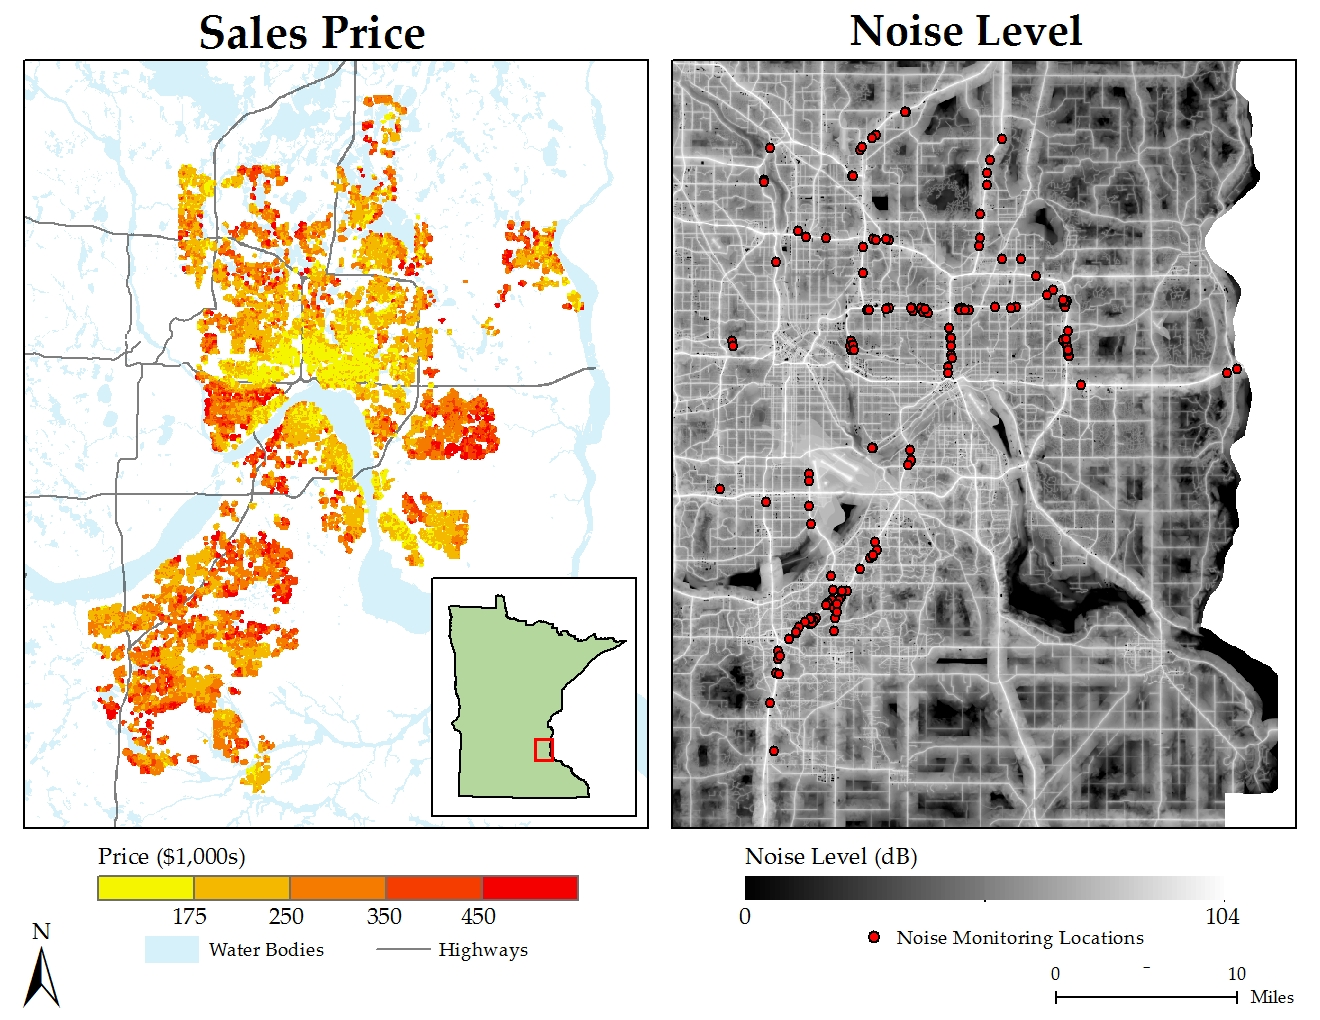
\includegraphics[width = 1.2\textwidth]{../graphs/Overview2column}}
\caption{This figure shows the spatial extent of our study area, the significant spatial variation in single family house sales prices, as well as our noise data.}\label{fig:overview}
\end{figure}

\begin{table}
\caption{Variable Description and Summary Statistics}\label{tab:sumStats}
\makebox[\linewidth][c]{
\small
\begin{tabular}{lD{.}{.}{1}D{.}{.}{1}D{.}{.}{1}D{.}{.}{1}D{.}{.}{1}D{.}{.}{1}D{.}{.}{1}}
  
 & min & 25\% & 50\% & mean & 75\% & max & st dev \\ 
  \hline
% latex table generated in R 2.15.2 by xtable 1.7-0 package
% Tue Jun 10 21:29:25 2014
Sale Price (\$1,000s) & 99 & 195 & 241 & 266 & 315 & 675 & 103 \\ 
  Year House was Built & 1850 & 1950 & 1973 & 1967 & 1993 & 2010 & 32 \\ 
  House Size (square feet) & 390 & 1158 & 1628 & 1750 & 2189 & 4000 & 704 \\ 
  Lot Size (acres) & 0.02 & 0.17 & 0.25 & 0.25 & 0.31 & 0.60 & 0.11 \\ 
  Owner Occupancy (Yes = 1, No = 0) & 0.0 & 1.0 & 1.0 & 0.8 & 1.0 & 1.0 & 0.4 \\ 
  Traffic Noise (dB) & 24.5 & 49.0 & 54.0 & 54.3 & 59.5 & 81.6 & 7.5 \\ 
  Distance to Central Business District (km) & 1.1 & 6.8 & 13.2 & 14.7 & 21.8 & 37.1 & 8.9 \\ 
  Distance to nearest Park (km) & 0.0 & 1.1 & 2.2 & 2.6 & 3.8 & 9.7 & 1.9 \\ 
  Distance to nearest Lake (km) & 0.0 & 0.4 & 0.8 & 0.9 & 1.3 & 4.4 & 0.7 \\ 
  Distance to nearest Shopping Center (km) & 0.0 & 0.9 & 1.5 & 1.9 & 2.3 & 10.8 & 1.6 \\ 
  Percent of Census Block Population Race = White & 0 & 80 & 90 & 85 & 96 & 100 & 17 \\ 
  Percent of Census Block Population Under Age 18 & 0 & 21 & 27 & 27 & 33 & 67 & 9 \\ 
  Median Income in Census Tract (\$1,000s) & 14 & 55 & 69 & 73 & 90 & 143 & 24 \\ 
  Elementary Test Scores & 336 & 360 & 365 & 364 & 370 & 552 & 11 \\ 
   \hline
\end{tabular}
}
\end{table}

\begin{table}
\caption{Matrix of Pearson Correlation Coefficients for Quantitative Variables}\label{tab:cor}
%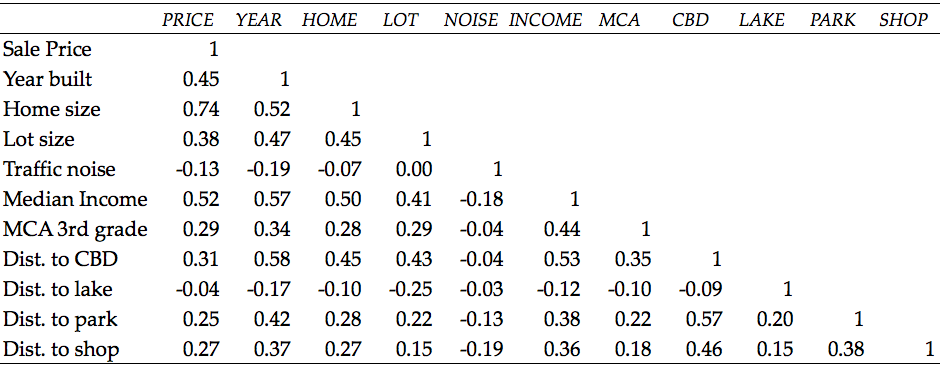
\includegraphics[width = \textwidth]{../graphs/CorrelationMatrix}
\begin{center}
\small
\tabcolsep=0.05cm
\makebox[\linewidth][c]{
\begin{tabular}{l|rrrrrrrrrrrrr}
 & \multicolumn{1}{x{.35in}}{Price} & \multicolumn{1}{x{.38in}}{House} & \multicolumn{1}{x{.35in}}{Lot} & 
 \multicolumn{1}{x{.35in}}{Built} & \multicolumn{1}{x{.35in}}{Noise} & \multicolumn{1}{x{.35in}}{CBD} & \multicolumn{1}{x{.35in}}{Park} & \multicolumn{1}{x{.35in}}{Lake} & \multicolumn{1}{x{.35in}}{Shop} & \multicolumn{1}{x{.35in}}{White} & 
 \multicolumn{1}{x{.35in}}{U18} & \multicolumn{1}{x{.35in}}{Inc.} & 
 \multicolumn{1}{x{.35in}}{Test} \tabularnewline 
  \hline
Sale Price & 1 &  &  &  &  &  &  &  &  &  &  &  &  \tabularnewline
House Size & 0.74 & 1 &  &  &  &  &  &  &  &  &  &  &  \tabularnewline
Lot Size  & 0.38 & 0.45 & 1 &  &  &  &  &  &  &  &  &  &  \tabularnewline
Year Built  & 0.45 & 0.52 & 0.47 & 1 &  &  &  &  &  &  &  &  &  \tabularnewline
Noise & -0.24 & -0.12 & -0.04 & -0.25 & 1 &  &  &  &  &  &  &  &  \tabularnewline
Distance to CBD  & 0.31 & 0.45 & 0.43 & 0.58 & -0.09 & 1 &  &  &  &  &  &  &  \tabularnewline
Distance to Park  & 0.25 & 0.28 & 0.22 & 0.42 & -0.17 & 0.57 & 1 &  &  &  &  &  &  \tabularnewline
Distance to Lake & -0.04 & -0.10 & -0.25 & -0.17 & -0.01 & -0.09 & 0.20 & 1 &  &  &  &  &  \tabularnewline
Distance to Shop  & 0.27 & 0.27 & 0.15 & 0.37 & -0.24 & 0.46 & 0.38 & 0.15 & 1 &  &  &  &  \tabularnewline
Percent White & 0.24 & 0.15 & 0.25 & 0.15 & -0.09 & 0.34 & 0.16 & -0.14 & 0.14 & 1 &  &  &  \tabularnewline
Percent Under 18 & 0.26 & 0.30 & 0.11 & 0.36 & -0.19 & 0.29 & 0.32 & 0.09 & 0.32 & -0.22 & 1 &  &  \\ 
Income & 0.52 & 0.50 & 0.41 & 0.57 & -0.24 & 0.53 & 0.38 & -0.12 & 0.36 & 0.35 & 0.32 & 1 &  \tabularnewline
Elem.\ Test Scores & 0.29 & 0.28 & 0.29 & 0.34 & -0.09 & 0.35 & 0.22 & -0.10 & 0.18 & 0.31 & 0.10 & 0.44 & 1 \tabularnewline 
\end{tabular} }
\end{center} 
\end{table}

\subsection{Noise Data}
To determine the relationship between real estate price and road traffic noise levels, we first created a traffic noise exposure surface by calculating the propagation of traffic noise over the landscape using the FHWA (Federal Highway Authority) 1978 standard \citep{Barry1978}. The entire methodology has already been explained in detail in (CITE two NEGA PAPERS) What follows is a summary. The modeling of traffic noise has three key components: choosing the mathematical function for noise propagation, assembling the input data, and assessing the accuracy of the model prediction. These will be briefly discussed.  Because it is currently used by the state of Minnesota, we used the FHWA 1978 standard model for calculating the noise level.  According to this standard, the noise level at any given location on the landscape can be expressed:  
\begin{eqnarray}\label{eq:noise}
L_{EQ}(i) &=& \bar{L}_0(i) + 0.115 \sigma _i^2 + 10 log \frac{N_i \pi D_0}{T*S_i} + 10 log \left[ \frac{D_0}{D}\right]^{1 + \alpha}  \nonumber \\
&& + 10 log \left( \frac{\psi _{\alpha (\phi _1, \phi _2)}}{\pi}\right) + \Delta _{gradient} + \Delta _{shielding}
\end{eqnarray}
where $L_{EQ}(i)$ is A-weighted hourly energy equivalent noise level in decibels (dBA), which is calculated for each class $i$ of vehicle (automobile and trucks); $\bar{L}_0(i)$ is the mean Sound Pressure Level (SPL) at the reference distance for class $i$; $\sigma _i$ is the standard deviation of the SPL for each class of vehicle; $N_i$ is the number of vehicles of the $i^{th}$ class passing during the relevant hour; $D_0$ is the reference distance (usually 15 m); $D$ is the perpendicular distance from the road center line to the receiver; $\alpha$ is a site parameter (soft and hard surface), $0 < \alpha < 1$; $S_i$ is the mean speed of the $i^{th}$ class; $T$ is the duration, usually 1 hour; $\phi _1$ and $\phi _2$ are the angles from the perpendicular of the limits of the observer's view of a section of the road. They are used to account for only the energy coming from a portion of the roadway; $\Delta _{gradient}$ is an adjustment for road surface gradient; $\Delta _{shielding}$ is a shielding adjustment (land cover, buildings, noise barriers).

We used several data sources as inputs in the study.  A 2007 road centerline and the associated traffic characteristics (volume and proportion of trucks and vehicles) for the region were obtained from the Minnesota Department of Transportation (MNDoT).  We converted the posted speed of each road segment into a GIS layer.  We used three data sources for the shielding adjustment: buildings, foliage, and noise barriers.  We extracted the perimeter and height of 818,500 buildings using a combination of LiDAR data and aerial photography.  Foliage shielding is accounted by extracting forest polygons that are at least 10 m high and have an area $\geq 10,000 m^2$ from a 2005 land use and 2001 National Land Cover Data. We obtained a noise barrier layer from the MNDoT that contains the locations, width, and height of each noise barriers to account for its shielding effect. 

We used the SoundPlanTM noise modeling software to implement equation\ref{eq:noise}.  Predicted noise output is calculated at a grid resolution of 10 m$^2$.  We conducted a preliminary validation of the model output by comparing it with observed noise levels, which were sampled at 134 locations along a major highway. The relationship between the mean observed and predicted noise levels was linear and moderately strong with a correlation of 0.76.

In order to incorporate noise produced by aircraft into the overall noise exposure, we obtained the aircraft noise contour lines of the region from the Twin Cities Metropolitan Airports Commission. The contour line noise values coincident with the traffic noise surface then were added following rules of logarithmic addition. For example, adding 52 dBA from aircraft contour line into the noise surface where the noise value is 51 yields 53.5 dBA. 

A map of our noise surface can be seen in Figure~\ref{fig:overview}. Once the noise surface for the entire region was developed, we extracted the noise surface for the present study area by overlaying the housing parcel boundaries and calculating the mean noise level within the parcel. 

\subsection{Structural Attributes}
According to a review by \cite{Wilhelmsson2000}, the five most common structural attributes included in real estate hedonic pricing studies are living area, number of bathrooms, age, garage and lot size.  The 2010 MetroGIS Regional Parcel Dataset includes structural data on living area, age, garage presence, lot size, owner-occupancy and house architectural style for every transaction. However, standard additional control variables like the number of bathrooms, bedrooms, and size of garage were not available through this source. We were able to obtain additional data for the number of bedrooms, bathrooms, and size of the garage for a subset of our house sales from the Dakota County Assessor's Office. In section \ref{Discussion} we show that the inclusion of these variables in our model does not significantly change our results for these areas. Therefore, we feel confident in our results even without these independent variables for most of our study area. %Additionally, other hedonic work has been published using a similar set of explanatory variables in this area, see for instance, \citet{Sander2009b}.

\subsection{Other Locational Attributes}
A common real estate adage states that the three most important real estate attributes are: location, location and location. Knowing where each house is located allows us to also construct a vector of other attributes associated with the sales transaction. For instance, using GIS software we are able to calculate the Euclidean distance to numerous points of interest within the dataset, such as the nearest central business district, shopping centers, parks, and lakes. Additionally, three demographic variables denoting the median household income for the surrounding census tract, the percentage of the population that identified their race as ``white'', and the percentage of the population that is under the age of 18 were created through the use of TIGER shapefiles from the 2010 Census Bureau and data from the 2010 American Community Survey. Lastly, we associate each transaction with its elementary school and include the average 3rd grade Minnesota Comprehensive Assessment (MCA) score for the local elementary school during the year of purchase.\footnote{Test scores were obtained from the Minnesota Department of Education website. The school district and elementary school attendance boundary spatial information were obtained from the Minnesota Geospatial Information Office Clearinghouse Data Catalog.} 

\subsection{Time}
We have sales transactions across six years (from 2005 to 2010) for our study area. Such temporal variation will allow us to estimate the hedonic price function over time and test for differences before, during, and after the economic recession. Table \ref{tab:SumStatsTime} displays the mean variable values by year of sale to look for differences over time. The mean sale price in 2009 (roughly \$230,000) is almost 20 percent lower than the mean sale price in 2006 (roughly \$280,000) and the number of sales transactions in 2009-10 is less than the number of transactions in 2005. However, most other variables have small or no differences across time. 

\begin{table}
\caption{Mean Variable Values by Year}\label{tab:SumStatsTime}
\makebox[\textwidth][c]{
\scriptsize
  \centering
    \begin{tabular}{lD{.}{.}{1}D{.}{.}{1}D{.}{.}{1}D{.}{.}{1}D{.}{.}{1}D{.}{.}{1}|D{.}{.}{1}}
    \\[-1.8ex]\hline 
\hline \\[-1.8ex] 
    & \multicolumn{6}{c}{Year of House Sale} & \\
    Variable & 2005 & 2006 & 2007 & 2008 & 2009 & 2010 & \multicolumn{1}{r}{All Years}\\ \hline
Sale Price (\$1,000s) & 279 & 282 & 275 & 262 & 231 & 233 & 266 \\ 
  Year House was Built & 1967 & 1966 & 1966 & 1971 & 1968 & 1968 & 1967 \\ 
  House Size (feet$^2$) & 1737 & 1736 & 1743 & 1813 & 1727 & 1775 & 1750 \\ 
  Lot Size (acres) & 0.25 & 0.25 & 0.25 & 0.26 & 0.25 & 0.26 & 0.25 \\ 
  Owner Occ (Y = 1, N = 0) & 0.87 & 0.87 & 0.92 & 0.86 & 0.60 & 0.77 & 0.83 \\ 
  Traffic Noise (dB) & 54.4 & 54.5 & 54.6 & 53.7 & 54.0 & 54.0 & 54.3 \\ 
  Dist CBD (km) & 14.7 & 14.6 & 14.8 & 15.0 & 14.3 & 14.5 & 14.7 \\ 
  Dist to  Park (km) & 2.6 & 2.6 & 2.6 & 2.8 & 2.6 & 2.6 & 2.6 \\ 
  Dist to Lake (km) & 0.9 & 0.9 & 0.9 & 0.9 & 0.9 & 0.9 & 0.9 \\ 
  Dist to  Shop (km) & 1.9 & 1.9 & 1.8 & 2.0 & 1.9 & 1.9 & 1.9 \\ 
  Percent Race = White & 84 & 84 & 85 & 86 & 85 & 86 & 85 \\ 
  Percent Under Age 18 & 28 & 28 & 27 & 28 & 27 & 27 & 27 \\ 
  Income (\$1,000s) & 72 & 72 & 72 & 75 & 73 & 73 & 73 \\ 
  Elementary Test Scores & 365 & 365 & 365 & 364 & 362 & 366 & 364 \\  \hline
  Number of Observations &  10,990  & 8,885  &  6,549  & 5,498  &  5,961  & 4,200  & 42,083  \\
    \end{tabular}%
}
\end{table}

We also created univariate density plots of the variables over time to check for differences in the shape or spread of the distributions over time (see Figure~\ref{fig:DensityPlots}). It is not the case that after the recession the distribution ``hollowed out'' in the middle and became bimodal with many high- and low-priced houses selling with few mid-priced homes selling. Additionally, maps of the locations of sales transactions over time reveal no discernable patterns, either (see Figure~\ref{fig:SalesYear}). The geographic dispersion of sales in earlier years looks surprisingly similar to that of later years. Thus, we can find no evidence of only certain types or locations of houses transacting in later years compared to earlier years in our data.

\begin{figure}
\makebox[\textwidth][c]{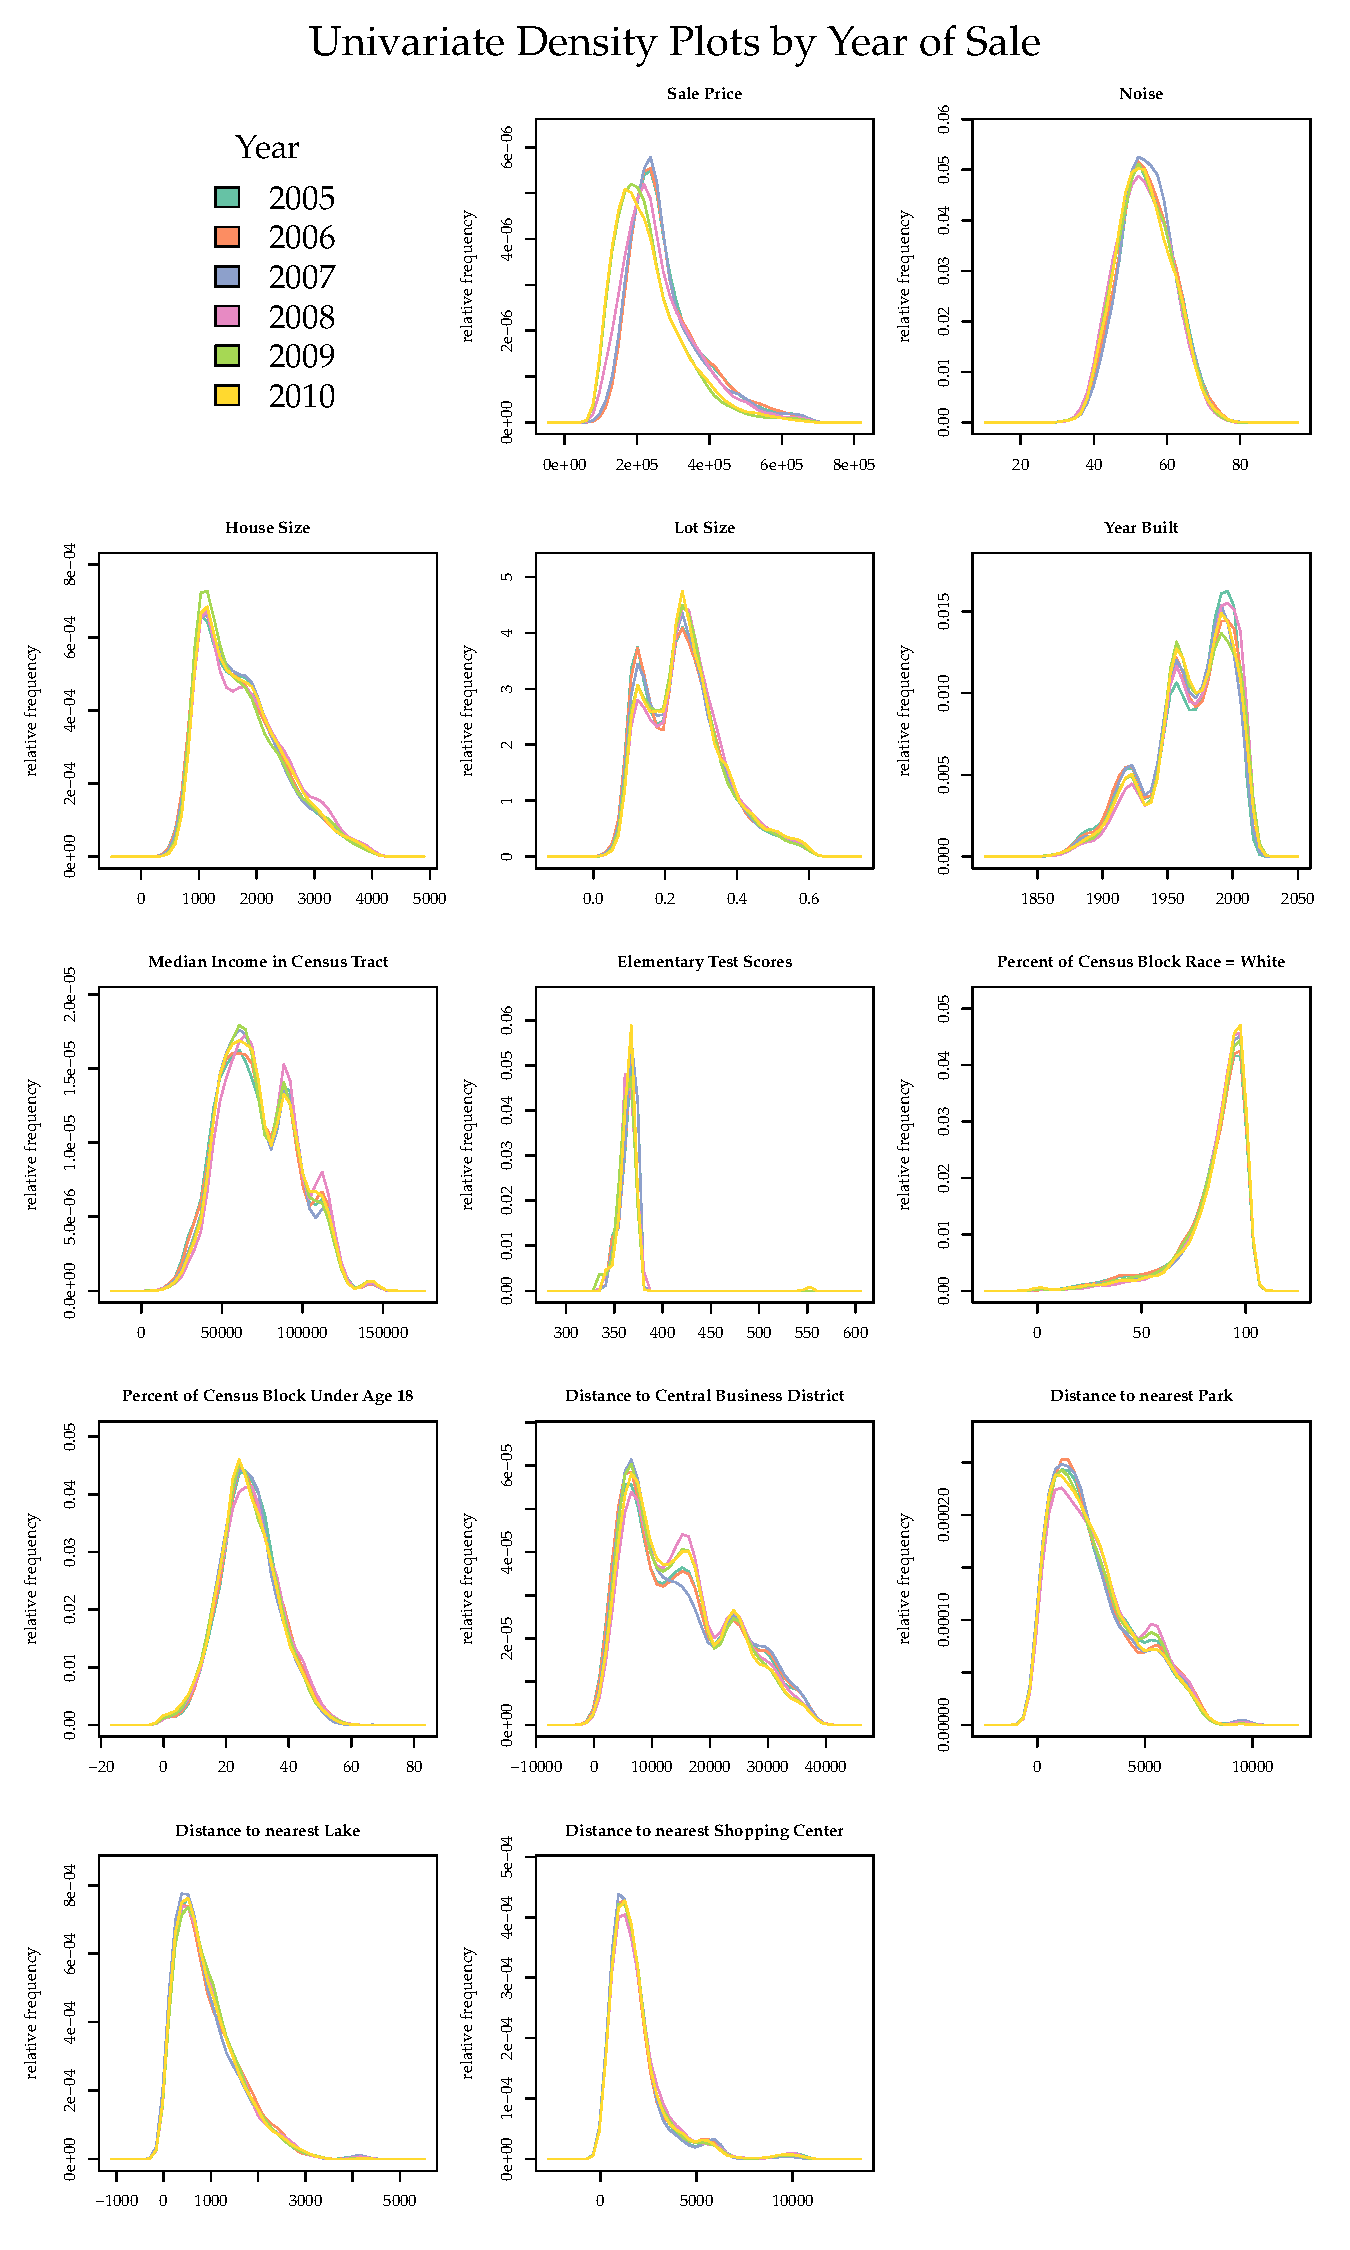
\includegraphics[width = \textwidth]{../graphs/DensityPlotsByYear}}
\caption{This figure shows }\label{fig:DensityPlots}
\end{figure}

\begin{figure}
\makebox[\textwidth][c]{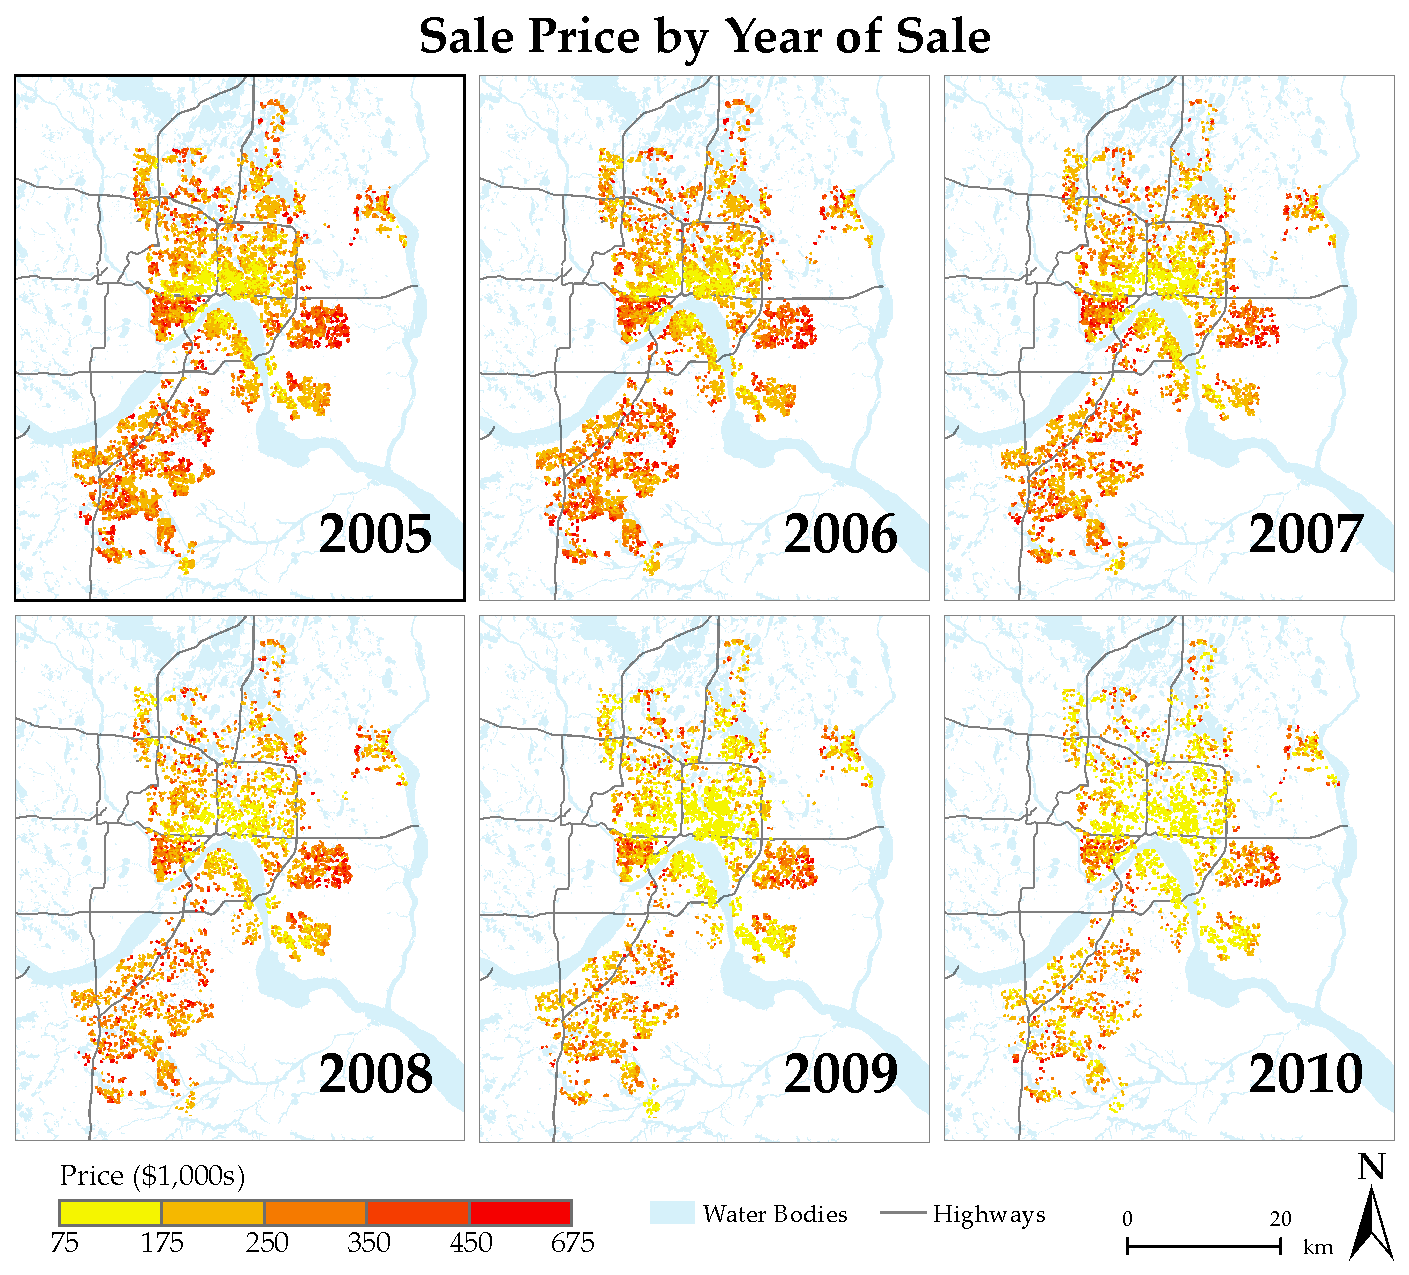
\includegraphics[width = \textwidth]{../graphs/SaleValue_with05}}
\caption{This figure shows }\label{fig:SalesYear}
\end{figure}

\section{Basic Econometric Model}\label{basicModel}
Our aim is to estimate the marginal willingness to pay for different attributes, in particular changes in the traffic noise associated with the house. Consistent with past research, this study implements a semi-logarithmic hedonic pricing model.  Before implementing the Locally Weighted Regression model, we present the results of a simpler econometric model given by equation~\eqref{eq:model}.
\begin{equation}\label{eq:model}	
ln \textrm{ Sale Price}_i = \beta _0 + \beta _1 \textrm{Noise}_i+ \beta _2 S_i+ \beta _3 N_i + \beta _4 T_i + \textrm{error}_i
\end{equation}
Noise$_i$ is the noise level for house $i$, $S_i$ is a vector of the house's structural attributes, $N_i$ is a vector of the neighborhood attributes, and $T_i$ is a vector of time fixed effects. Due to the semi-logarithmic functional form of the model, we can interpret the regression model coefficients as the price semi-elasticities of the underlying attributes. For instance, we can interpret the coefficient on noise as the percentage increase in price for a one decibel increase in the traffic noise associated with the transaction in our dataset. 


\begin{table}
\caption{Basic Global Regression Results}\label{tab:globalRegression}
\makebox[\textwidth][c]{
\scriptsize
  \centering
\begin{tabular}{@{\extracolsep{-1pt}}lD{.}{.}{-4} D{.}{.}{-4} D{.}{.}{-4} D{.}{.}{-4} } 
\\[-1.8ex]\hline 
\hline \\[-1.8ex] 
 & \multicolumn{4}{c}{\textit{Dependent variable: ln Sale Price}} \\ 
\cline{2-5} \\[-1.8ex] 
& \multicolumn{1}{r}{Model (A)} & \multicolumn{1}{r}{Model (B)} & \multicolumn{1}{r}{Model (C)} & \multicolumn{1}{r}{Model (D)}\\ 
& \multicolumn{1}{r}{All Years} & \multicolumn{1}{r}{Year=2006} & \multicolumn{1}{r}{Year=2008} & \multicolumn{1}{r}{Year=2010}\\
\hline \\[-1.8ex] 
Noise (dB) & -0.0027^{***} & -0.0020^{***} & -0.0033^{***} & -0.0040^{***} \\ 
  & (0.0001) & (0.0003) & (0.0005) & (0.0006) \\ 
  & & & & \\ 
 House Size (1,000s ft$^2$) & 0.2914^{***} & 0.2847^{***} & 0.2810^{***} & 0.3066^{***} \\ 
  & (0.0022) & (0.0043) & (0.0067) & (0.0084) \\ 
  & & & & \\ 
 Lot Size (acres) & 0.2493^{***} & 0.2719^{***} & 0.2799^{***} & 0.2135^{***} \\ 
  & (0.0118) & (0.0221) & (0.0359) & (0.0447) \\ 
  & & & & \\ 
 Owner Occupancy Dummy & 0.0222^{***} & -0.0027 & 0.0478^{***} & 0.0298^{***} \\ 
  & (0.0026) & (0.0050) & (0.0085) & (0.0097) \\ 
  & & & & \\ 
 Year House Built & 0.0020^{***} & 0.0025^{***} & 0.0018^{***} & 0.0011^{***} \\ 
  & (0.0001) & (0.0001) & (0.0002) & (0.0002) \\ 
  & & & & \\ 
 Percent Under 18 & -0.0001 & 0.00002 & -0.0002 & -0.0006 \\ 
  & (0.0001) & (0.0002) & (0.0004) & (0.0005) \\ 
  & & & & \\ 
 Percent White & 0.0037^{***} & 0.0031^{***} & 0.0040^{***} & 0.0040^{***} \\ 
  & (0.0001) & (0.0001) & (0.0002) & (0.0003) \\ 
  & & & & \\ 
 Median Income (\$1,000s) & 0.0023^{***} & 0.0021^{***} & 0.0023^{***} & 0.0029^{***} \\ 
  & (0.0001) & (0.0001) & (0.0002) & (0.0003) \\ 
  & & & & \\ 
 Elementary Test Scores & 0.0009^{***} & 0.0023^{***} & 0.0040^{***} & 0.0001 \\ 
  & (0.0001) & (0.0003) & (0.0005) & (0.0002) \\ 
  & & & & \\ 
 Dist to CBD (km) & 0.0078^{***} & 0.0083^{***} & 0.0053^{***} & 0.0101^{***} \\ 
  & (0.0005) & (0.0010) & (0.0016) & (0.0020) \\ 
  & & & & \\ 
 Dist to Lake (km) & 0.0230^{***} & 0.0246^{***} & 0.0021 & 0.0343^{***} \\ 
  & (0.0017) & (0.0032) & (0.0054) & (0.0067) \\ 
  & & & & \\ 
 Dist to Park (km) & 0.0014 & -0.0027 & 0.0099^{***} & 0.0064^{*} \\ 
  & (0.0009) & (0.0017) & (0.0027) & (0.0034) \\ 
  & & & & \\ 
 Dist to Shop (km) & -0.0019^{*} & -0.0020 & -0.0063^{*} & -0.0020 \\ 
  & (0.0010) & (0.0019) & (0.0033) & (0.0041) \\ 
  & & & & \\ 
\hline \\[-1.8ex] 
Home Style Fixed Effects & \multicolumn{1}{c}{Yes} & \multicolumn{1}{c}{Yes} & \multicolumn{1}{c}{Yes} & \multicolumn{1}{c}{Yes} \\ 
Month*Year Fixed Effects & \multicolumn{1}{c}{Yes} & \multicolumn{1}{c}{Yes} & \multicolumn{1}{c}{Yes} & \multicolumn{1}{c}{Yes} \\ 
City Fixed Effects & \multicolumn{1}{c}{Yes} & \multicolumn{1}{c}{Yes} & \multicolumn{1}{c}{Yes} & \multicolumn{1}{c}{Yes} \\ 
\hline \\[-1.8ex] 
Observations & \multicolumn{1}{c}{42,083} & \multicolumn{1}{c}{8,885} & \multicolumn{1}{c}{5,498} & \multicolumn{1}{c}{4,200} \\ 
R$^{2}$ & \multicolumn{1}{c}{0.742} & \multicolumn{1}{c}{0.785} & \multicolumn{1}{c}{0.691} & \multicolumn{1}{c}{0.668} \\ 
\hline 
\hline \\[-1.8ex] 
\textit{Note:}  & \multicolumn{4}{r}{$^{*}$p$<$0.1; $^{**}$p$<$0.05; $^{***}$p$<$0.01} \\ 
\end{tabular} 
}
\end{table}

Model (A) in Table \ref{tab:globalRegression} displays the results of a basic Ordinary Least Squares regression model. In addition to the important structural and neighborhood variables, we also include fixed effects for each city and month of sale in the dataset to allow for month-to-month shocks to prices. The traffic noise coefficient suggests houses in our data that are similar in all respects but a one decibel difference in noise will, on average, have sales prices roughly 0.27 percent lower at the noisier location.  

Further exploratory analysis suggests the assumption of temporal and geographic stationarity of the hedonic price function is overly restrictive and needs to be relaxed. We first tested for temporal changes in the coefficients for house size, lot size, and noise by creating interaction terms with these variables and the month*year year fixed effects. In all three cases the improved model fit was significantly more than expected due to random chance.\footnote{The results of specific hypothesis tests are available upon request.} Columns (B) - (D) of Table \ref{tab:globalRegression} show the results of restimating Model (A) using only sales within three separate years of data. Subsequent analysis also suggests that many of the important regression coefficients vary across the different cities within our data. We are able to reject the null hypothesis that the interaction terms between cities and important variables (house size, lot size, noise, etc.) are zero, even after limiting the analysis to only houses sold within a given year (for instance, by adding the interaction terms to model specifications (B) - (D)).\footnote{Results of specific F-tests are available upon request.} 

These results should be taken with appropriate skepticism, as the models are simple Ordinary Least Squares regressions and the spatial and temporal nature of the data likely violate assumptions of the Classical Linear Regression Model. However, the initial findings seem to suggest that the relationship between house prices and many other hedonic characteristics may vary over space and time. While methods exist for parameterizing this variation \citep[such as spatial expansion as suggested by][]{Casetti1972}, we have no a priori knowledge of how to parameterize the variation. As such, we turn to a semi-parametric form of hedonic regression, a flexible modeling approach which lets the data reveal how relationships vary, rather than specifying them beforehand. Such a modeling choice will allow us to perform additional tests of the hypotheses of spatial and temporal stationarity in the regression model.

\section{Locally Weighted Regression Model}
Locally Weighted Regression (LWR) techniques (also known as Geographically Weighted Regression) are described in detail by \citet{Cleveland1988}, \citet{Brunsdon1998b}, \citet{Fotheringham2002}, and others. It is a weighted least squares methodology in which regression coefficients are estimated over space as a function of the local data as described in Equation~\eqref{eq:LWRbeta},
\begin{equation}\label{eq:LWRbeta}
\hat{\beta}_i = (X'W_iX)^{-1}X'W_iY,
\end{equation}
where X is a $n \times m$ matrix of independent variables, $W_i$ is the $n \times n$ weights matrix, and Y is the $n \times 1$ vector of dependent variable values. The weights matrix, $W_i$ is a diagonal matrix where element $w_{jj}$ denotes the weight that the $j^{th}$ data point will receive in the regression coefficients estimated at location $i$ in the dataset. We employ a bi-square weights function and a k-nearest neighbor bandwidth approach as described in equation~\eqref{eq:weights}, 
\begin{equation}\label{eq:weights}
w_{jj}=\left[1-\left(\frac{d_{ij}}{d_{k}}\right)^2 \right]^2 \textrm{ if  }d_{ij}<d_{ik}\textrm{, otherwise = 0},
\end{equation}
where $d_{ij}$ denotes the distance between observations $i$ and $j$, and $d_{ik}$ is the distance from observation $i$ to the $k^{th}$ nearest observation. This function assigns weights close to 1 for data points near observation $i$, weights positive but closer to zero for observations farther away, and zero for all $n-k$ observations farther away than the $k^{th}$ nearest observation. We estimate LWR coefficients using bandwidths ranging from as small as $k=50$ observations and as large as 10,000 observations. We choose the LWR bandwidth my minimizing the Generalized Cross Validation score as detailed in equation~\eqref{eq:GCV},
\begin{equation}\label{eq:GCV}
n*\sum_{i=1}^{n}\frac{(y_i-\hat{y}_i)^2}{(n-v_1)^2}, 
\end{equation} 
where $y_i$ is the dependent variable value, $\hat{y}_i$ is the predicted dependent variable value for observation $i$, and $v_1$ is the ``effective number of model parameters.'' The value  
$v_1=$tr(\textbf{S}), where the matrix \textbf{S} is the ``hat matrix'' which maps $y$ onto $\hat{y}$,
                   \begin{equation*}
                   \hat{y}=\textbf{S}y,
                   \end{equation*}
                   and each row of \textbf{S}, $r_i$ is given by:
                     \begin{equation*}
                   r_i=X_i(X'W_iX)^{-1}X'W_i.
                   \end{equation*}
The GCV score is a convenient model selection metric that rewards models that provide a good fit to the data, while penalizing models with a greater number of model parameters \citep{Loader1999, McMillen2010}. Model selection via this strategy has been shown to discern whether spatially varying relationships exist, accurately estimate spatially varying coefficients, even outperform other spatial econometric techniques, and do so without wasting degrees of freedom \citep{Paez2011, McMillen2010, McMillen2012}. 

%\section{Results}
Similar to the basic econometric model described in Section \ref{basicModel}, the LWR model estimates the logged sales price of a house as a function of structural and neighborhood variables, location and time. In order to account for changing market conditions in our data as manifested in regression coefficients that vary over time, when estimating LWR coefficients we use only houses sold within the past 12 months and also include month fixed effects to account for seasonality. Thus, the coefficient estimates at a particular house are estimated using data from other sales nearby in both time and geography.

\subsection{Improved Model Performance}
The use of the Locally Weighted Regression model significantly increases model performance as measured by the generalized cross validation score. Figure \ref{fig:GCVmodel} displays the Generalized Cross Validation score for three different model specifications estimated at the ``global'' level as well as with varying numbers of observations included in the regression bandwidth. We estimate three different hedonic function specifications with different levels of additional spatial control variables. Model (1) includes the noise variable, the basic structural characteristics (size of the house in square feet, size of the lot in acres, a categorical variable denoting the architectural style of the house, and whether or not the house is owner-occupied) plus month of sale*year fixed effects. Model (2) includes all of the str adds neighborhood and locational variables to the previously described model (test scores at the local elementary school, census tract median income, percent of the census block population that is white, percentage of the census block that is under age 18 and distances to the central business district, nearest park, nearest shopping center, and nearest lake). The third model adds city fixed effects to the second model. Thus Model (3) explicitly includes both common important characteristics of neighborhood quality while also allowing for spatial heterogeneity in the regression coefficients, and even city-level fixed effects to control for omitted variables that vary at the municipal level.

Two important conclusions can be drawn from these results. Model (3) consistently outperforms the other two models-- slightly better than Model (2) and considerably better than Model (1). Thus, even conditional on having modeled the data with local regression, the inclusion of more neighborhood-level variables substantially improves the model fit. Second, local analyses perform significantly better than global models. The minimum GCV score is obtained using a bandwidth of 500 nearest houses and a model including structural, neighborhood, and locational variables in addition to time and city fixed-effects. 

\begin{figure}
  \makebox[\textwidth][c]{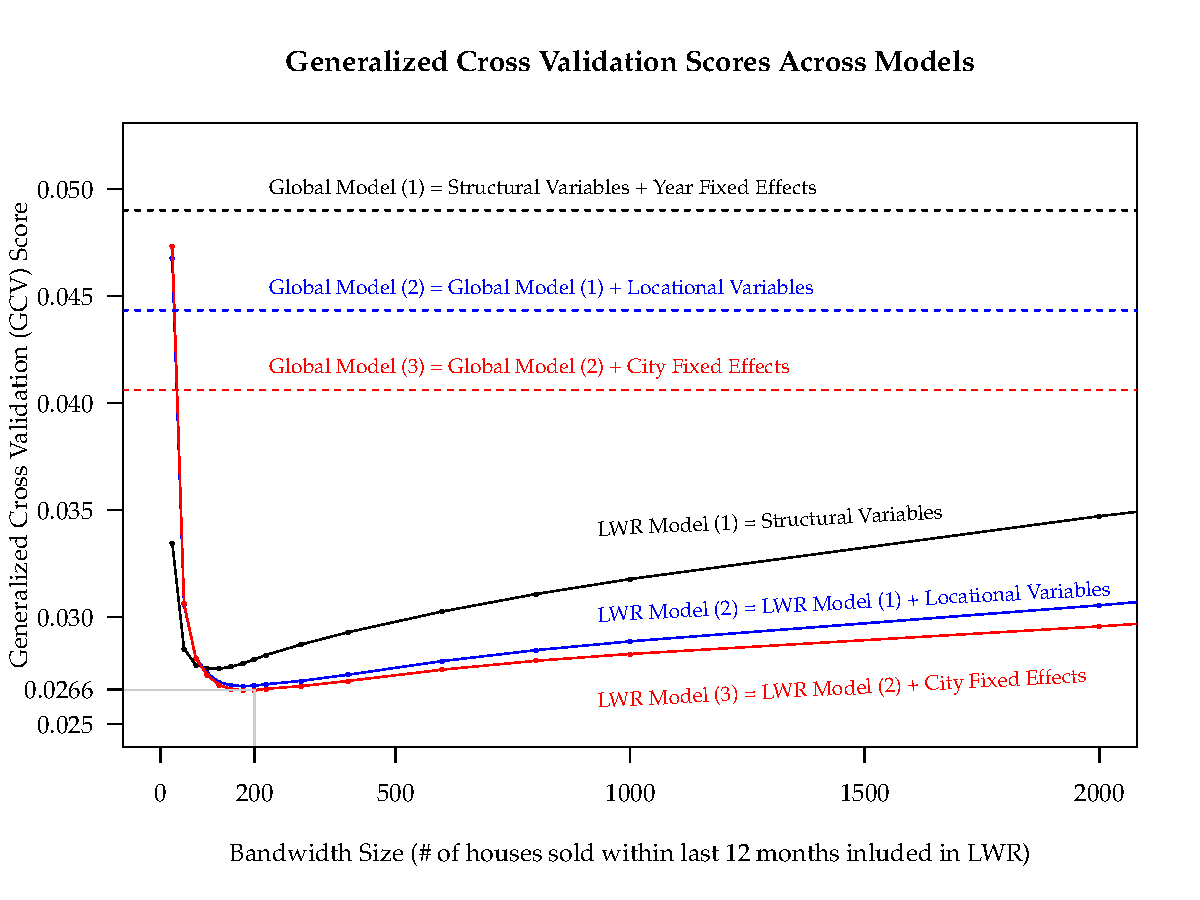
\includegraphics[width = 1.2\textwidth]{../graphs/GCVbyModel}}
\caption{This figure shows the relationship between bandwidth size and the GCV score for three different Locally Weighted Regression (LWR) models. For comparison, the GCV scores for each model when estimated at a global scale are also shown. Note that the LWR models all have significantly smaller GCV scores than the global models. The minimum GCV score is obtained by LWR Model (3) at a bandwidth of 500 nearest houses.}\label{fig:GCVmodel}
\end{figure}

%Table \ref{tab:LWR} summarizes the results of LWR Model (3) at three different bandwidth sizes plus the same model estimated at the ``global'' level. run without allowing for spatial variation in the regression coefficients. Again, note that the LWR model yields a substantially smaller GCV score (0.027 vs.\ 0.038) signifying a substantial improvement in model performance. In addition to the significant reduction in the GCV score obtained with the use of LWR, we also see a substantial reduction in the degree of spatial autocorrelation in the model residuals. We calculate Moran's I statistic to be 0.199 for the global model while our preferred LWR specification yields 0.012, a more than ten-fold reduction. 


% Table created by stargazer v.5.1 by Marek Hlavac, Harvard University. E-mail: hlavac at fas.harvard.edu
% Date and time: Sat, Jun 21, 2014 - 10:37:00 AM
% Requires LaTeX packages: dcolumn 
\begin{table}[!htbp]
  \caption{LWR Results: Dependent Variable = ln(Sales Price)} 
  \label{tab:LWR} 
  \makebox[\textwidth][c]{
\scriptsize
  \centering
\begin{tabular}{@{\extracolsep{-1pt}} D{.}{.}{4} D{.}{.}{4} D{.}{.}{4} D{.}{.}{4} D{.}{.}{-4} D{.}{.}{4} D{.}{.}{4} D{.}{.}{-4} D{.}{.}{3} D{.}{.}{3} } 
\\[-1.8ex]\hline 
\hline \\[-1.8ex]
 & \multicolumn{3}{c}{Nearest 500 sales$^*$} & \multicolumn{3}{c}{Nearest 650 sales} & \multicolumn{3}{c}{Nearest 1000 sales} \\
 & \multicolumn{1}{r}{mean $\hat{\beta}$} & \multicolumn{1}{c}{10$^{th}$} & \multicolumn{1}{c}{90$^{th}$}  & 
 \multicolumn{1}{r}{mean $\hat{\beta}$} & \multicolumn{1}{c}{10$^{th}$} & \multicolumn{1}{c}{90$^{th}$}  & 
 \multicolumn{1}{r}{mean $\hat{\beta}$} & \multicolumn{1}{c}{10$^{th}$} & \multicolumn{1}{c}{90$^{th}$} \\
 \cline{2-4} \cline{8-10} \cline{5-7}
\multicolumn{1}{l}{Noise (dB)} & -0.0034 & -0.0064 & -0.0006 & -0.0034 & -0.0061 & -0.0009 & -0.0033 & -0.0057 & -0.0013 \\ 
\multicolumn{1}{l}{House Size (1,000s ft)} & 0.2700 & 0.1800 & 0.3900 & 0.2700 & 0.1900 & 0.3900 & 0.2700 & 0.2000 & 0.4000 \\ 
\multicolumn{1}{l}{Lot Size (acres)} & 0.4200 & 0.1700 & 0.7300 & 0.4200 & 0.1900 & 0.7100 & 0.4200 & 0.2100 & 0.6700 \\ 
\multicolumn{1}{l}{Year House Built} & 0.0046 & 0.0004 & 0.0100 & 0.0045 & 0.0005 & 0.0096 & 0.0043 & 0.0005 & 0.0090 \\ 
\multicolumn{1}{l}{Owner Occupancy} & 0.0230 & -0.0290 & 0.0800 & 0.0240 & -0.0240 & 0.0760 & 0.0230 & -0.0180 & 0.0680 \\ 
\multicolumn{1}{l}{Percent White} & 0.0012 & -0.0003 & 0.0029 & 0.0013 & -0.0001 & 0.0028 & 0.0014 & 0.0001 & 0.0028 \\ 
\multicolumn{1}{l}{Percent Under 18} & 0.0005 & -0.0016 & 0.0025 & 0.0004 & -0.0014 & 0.0022 & 0.0004 & -0.0011 & 0.0019 \\ 
\multicolumn{1}{l}{Median Income (\$1,000s)} & 0.0007 & -0.0014 & 0.0033 & 0.0008 & -0.0010 & 0.0033 & 0.0010 & -0.0006 & 0.0037 \\ 
\multicolumn{1}{l}{Elementary Test Scores} & 0.0000 & -0.0056 & 0.0055 & 0.0001 & -0.0050 & 0.0049 & 0.0003 & -0.0040 & 0.0042 \\ 
\multicolumn{1}{l}{Dist to Lake (km)} & -0.0150 & -0.0910 & 0.0580 & -0.0110 & -0.0770 & 0.0550 & -0.0076 & -0.0630 & 0.0520 \\ 
\multicolumn{1}{l}{Dist to Park (km)} & -0.0110 & -0.0600 & 0.0330 & -0.0110 & -0.0490 & 0.0250 & -0.0085 & -0.0370 & 0.0160 \\ 
\multicolumn{1}{l}{Dist to Shop (km)} & 0.0092 & -0.0330 & 0.0520 & 0.0096 & -0.0270 & 0.0470 & 0.0100 & -0.0210 & 0.0440 \\ 
\multicolumn{1}{l}{Dist to CBD (km)} & 0.0084 & -0.0190 & 0.0440 & 0.0094 & -0.0140 & 0.0400 & 0.0100 & -0.0099 & 0.0380 \\ 
\hline \\[-1.8ex] 
\multicolumn{10}{p{6 in}}{$^*$ A bandwidth of 500 implies that the nearest 500 houses sold within the past 12 months are included.} \\
\multicolumn{10}{p{6 in}}{Note: Each model also includes a categorical variable for architectural style, month*year fixed effects, and city-level fixed effects. }

\end{tabular} 
}
\end{table} 

Table~\ref{tab:LWR} shows the results for our LWR Model (3) with three different bandwidths: the GCV minimizing bandwidth of 500 nearest sales as well as two larger values, 650 and 1,000 nearest sales. For each bandwidth, we display the mean LWR coefficient as well as the 10$^{th}$ and 90$^{th}$ percentile values. The mean LWR coefficient for the noise variable is similar across the three different bandwidths (approximately a third of a percent difference in house sales prices for each additional decibel of noise, all other varibles held constant). Unsurprisingly, the spread of the coefficient distribution is greater for the smaller bandwidths. We now turn to investigating whether this increased dispersion appears from the stochastic nature of smaller sample sizes, or due to heterogeneity in the hedonic function.

We believe the hedonic function varies significantly over space and time and that the use of a LWR estimation procedure is an appropriate and beneficial modeling strategy. In the next three subsections we describe the results of hypothesis tests that lead us to these conclusions. 

\subsection{Does the Hedonic Function Vary over Space?}

We first conducted a Monte Carlo simulation recommended in \citet{Fotheringham2002} to see if the improved model fit with our LWR model was due to random chance. The intuition of the test is as follows - if the improved model fit isn't significant, then we should be able to see similar improvements in model fit by using the LWR model with the same houses but in a different spatial arrangement. Failing to recreate a spatial arrangement that yields a similar model fit as to that obtained with our actual data is then evidence that our spatial arrangement and the improved model fit obtained from a spatially heterogeneous model is significant. 

We conducted 100 different experiments in which we randomly swapped the locations of our house transactions. In each case we then estimated the LWR model using 10 different bandwidths ranging from the nearest 100 to 4,000 sales just as before and calculated the GCV score. Every single time the smallest Generalized Cross-Validation score was obtained at the largest bandwidth. That is, in 100 consecutive opportunities to fit our data at a local level of a couple hundred nearest sales up to a couple thousand nearby sales, the GCV score was always smallest for the largest possible bandwidth. In other words, after running a thousand different local regression models on the shuffled data, we never obtained model performance anywhere near the LWR model with our true locational data. This seems to be strong evidence that the increased ability to predict house prices with a local model is not due to chance and that there is spatial non-stationarity in the hedonic function.



\subsection{Which Coefficients Vary over Space?}

The previous section presented evidence in support of the claim that there exists significant spatial variation in the hedonic function. However, we have not yet established which variables have spatially varying coefficients. Figures~\ref{fig:AcreBetas} -- \ref{fig:NoiseBetas} show the spatial variation in the estimated LWR coefficients for three important variables, lot size, house size, and noise. For comparison, we present the results across four different levels of local analysis, ranging from LWR bandwidths of 500 nearest houses to the nearest 2,000 sales. 

A few patterns are clear in Figures~\ref{fig:AcreBetas} -- \ref{fig:NoiseBetas}. For instance, across all four bandwidths we see that the hedonic\footnote{Remember that the dependent variable is the log of sales price.} coefficient on lot size (measured in acres) is largest near the central business district of St.\ Paul. Thus, consistent with standard urban economic theory, to the extent that the hedonic coefficient is correlated with the price of land, our results suggest the price of land is highest near the central business district and declines with distance from the CBD. This tendency is consistent across the four different bandwidths presented (other specific results available upon request). The LWR coefficients on house size (measured in thousands of square feet of finished space) also seem to exhibit spatial variation across the different bandwidths. In the west-central portion of our study area (a collection of notably desirable neighborhoods) we see a cluster of large LWR coefficients, while those areas in the southernmost portion of our region (suburban areas) have the smallest coefficients. 

In Figure~\ref{fig:NoiseBetas} we map the estimated LWR noise coefficients from four different bandwidths. In this figure the red areas represent large negative coefficients, while yellow areas are characterized by values closer to zero. It is interesting to note that for the smaller bandwidths, the area with the most negative noise coefficients is ringed by some of the coefficients closest to zero (and even greater than zero in some cases). As the bandwidth increases to 1000 or 2000 nearest houses, the variation in noise coefficients decreases substantially. In contrast to the previous two figures, we have largely eliminated the ``hot spots'' that appear in the smaller bandwidths. 


\begin{figure}
 \makebox[\textwidth][c]{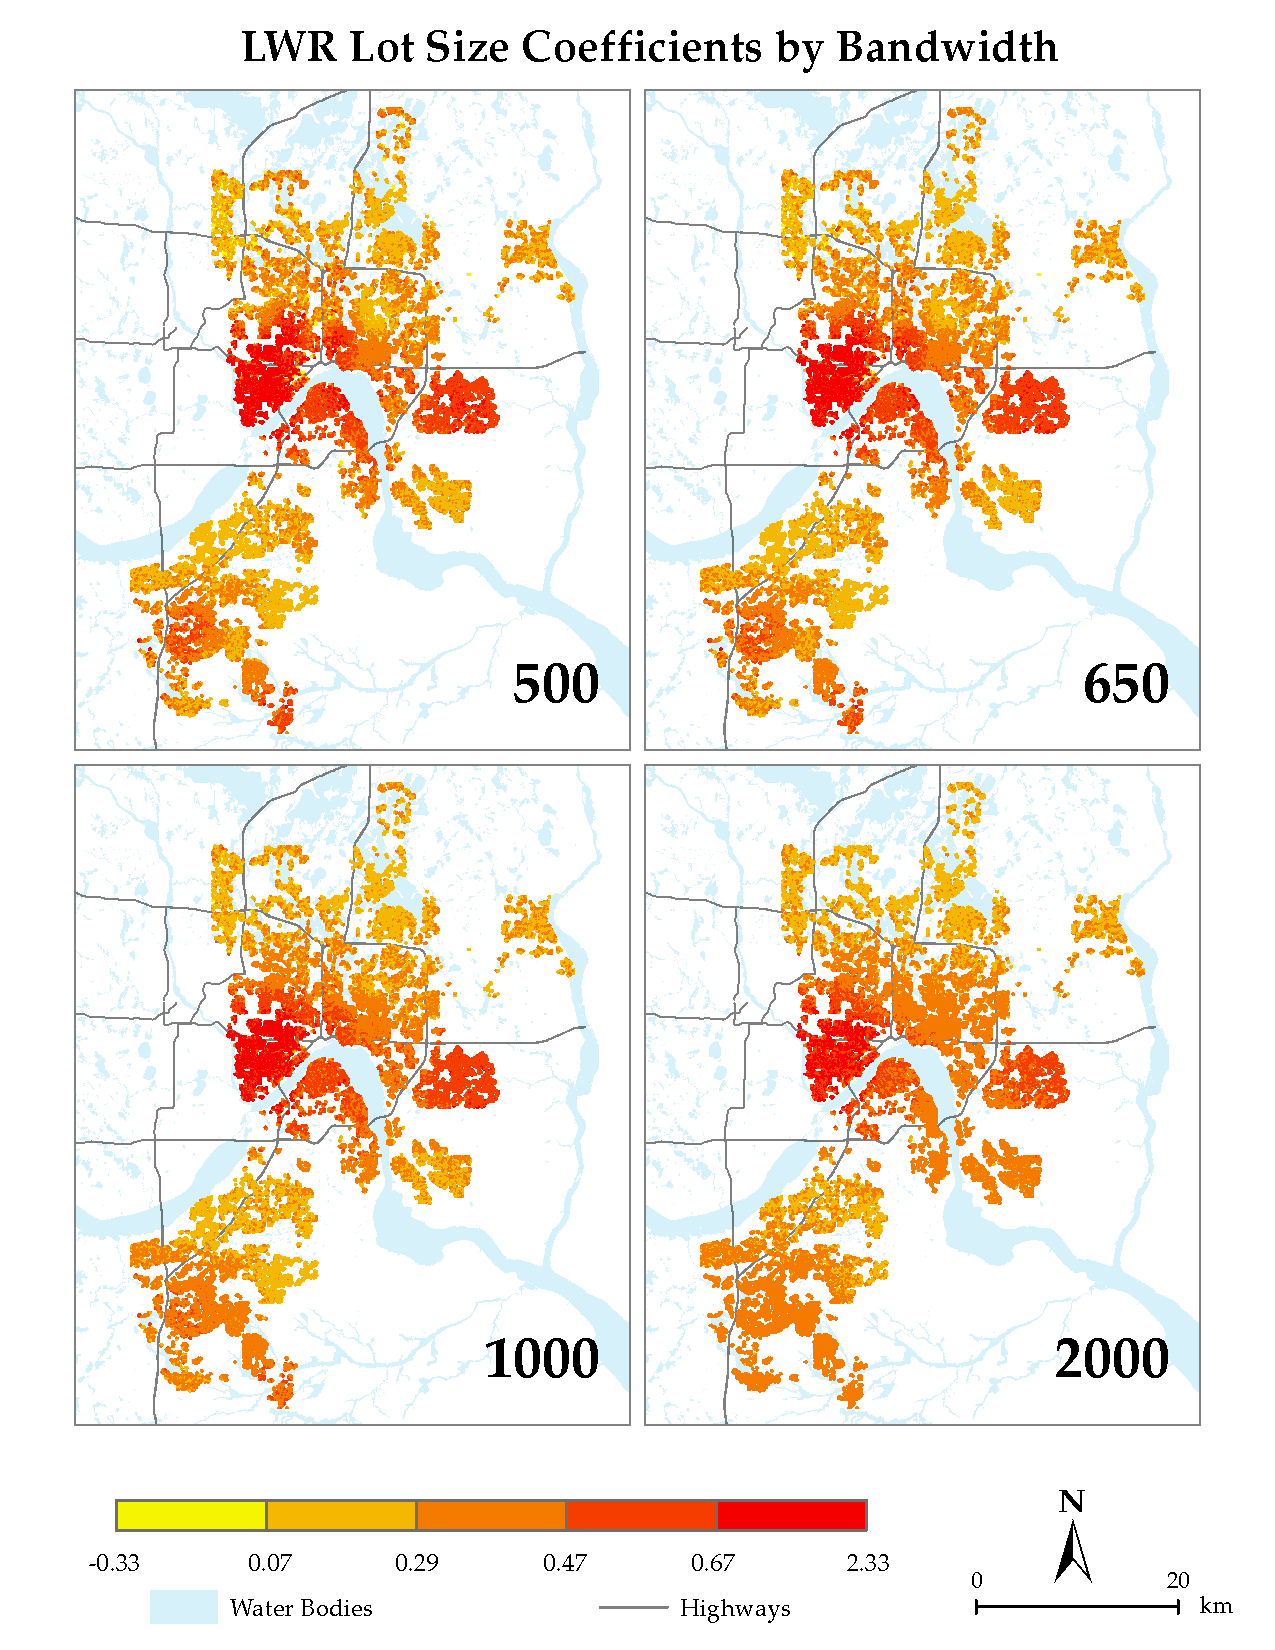
\includegraphics[width=1.1\textwidth]{../graphs/AcreBeta_allBandwidth}}
 \caption{Simula.}\label{fig:AcreBetas}
\end{figure}

\begin{figure}
 \makebox[\textwidth][c]{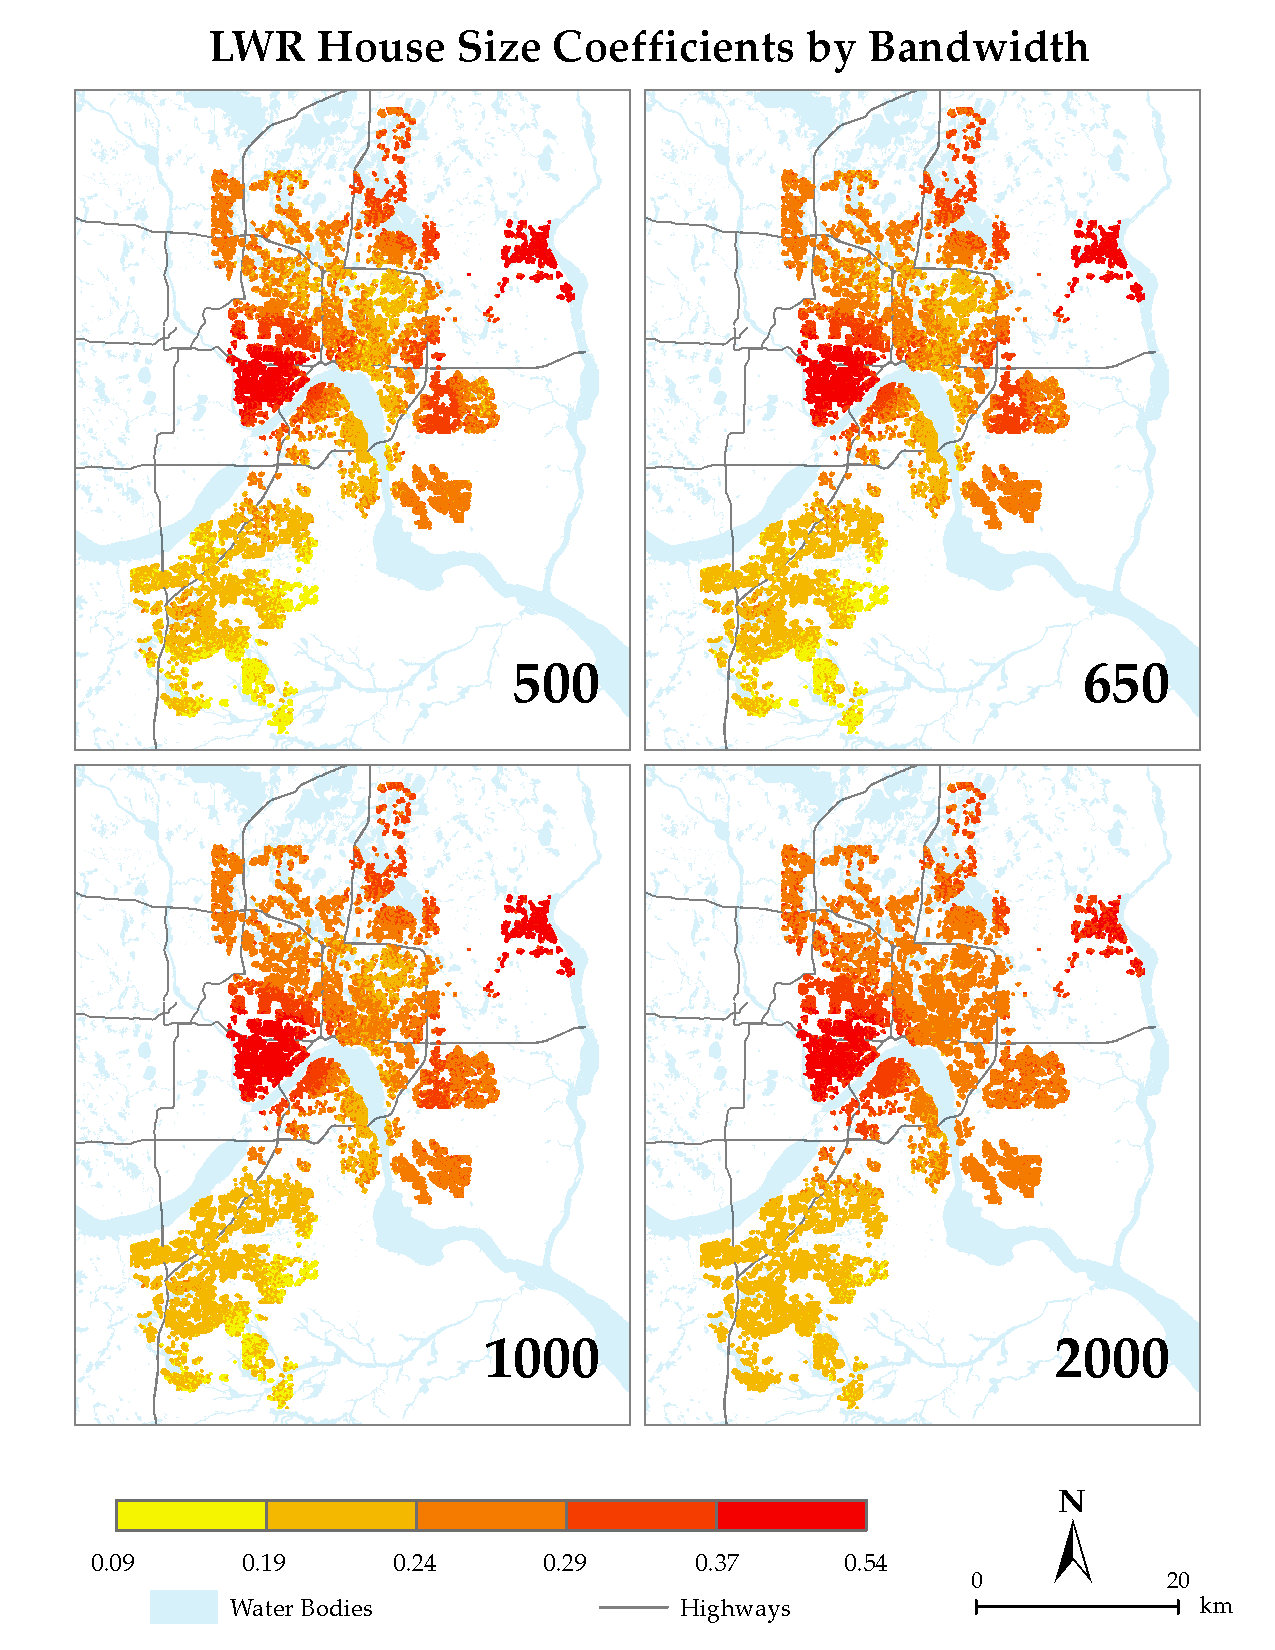
\includegraphics[width=1.1\textwidth]{../graphs/FinSqFtBeta_allBandwidth}}
 \caption{Simula.}\label{fig:HouseBetas}
\end{figure}


\begin{figure}
 \makebox[\textwidth][c]{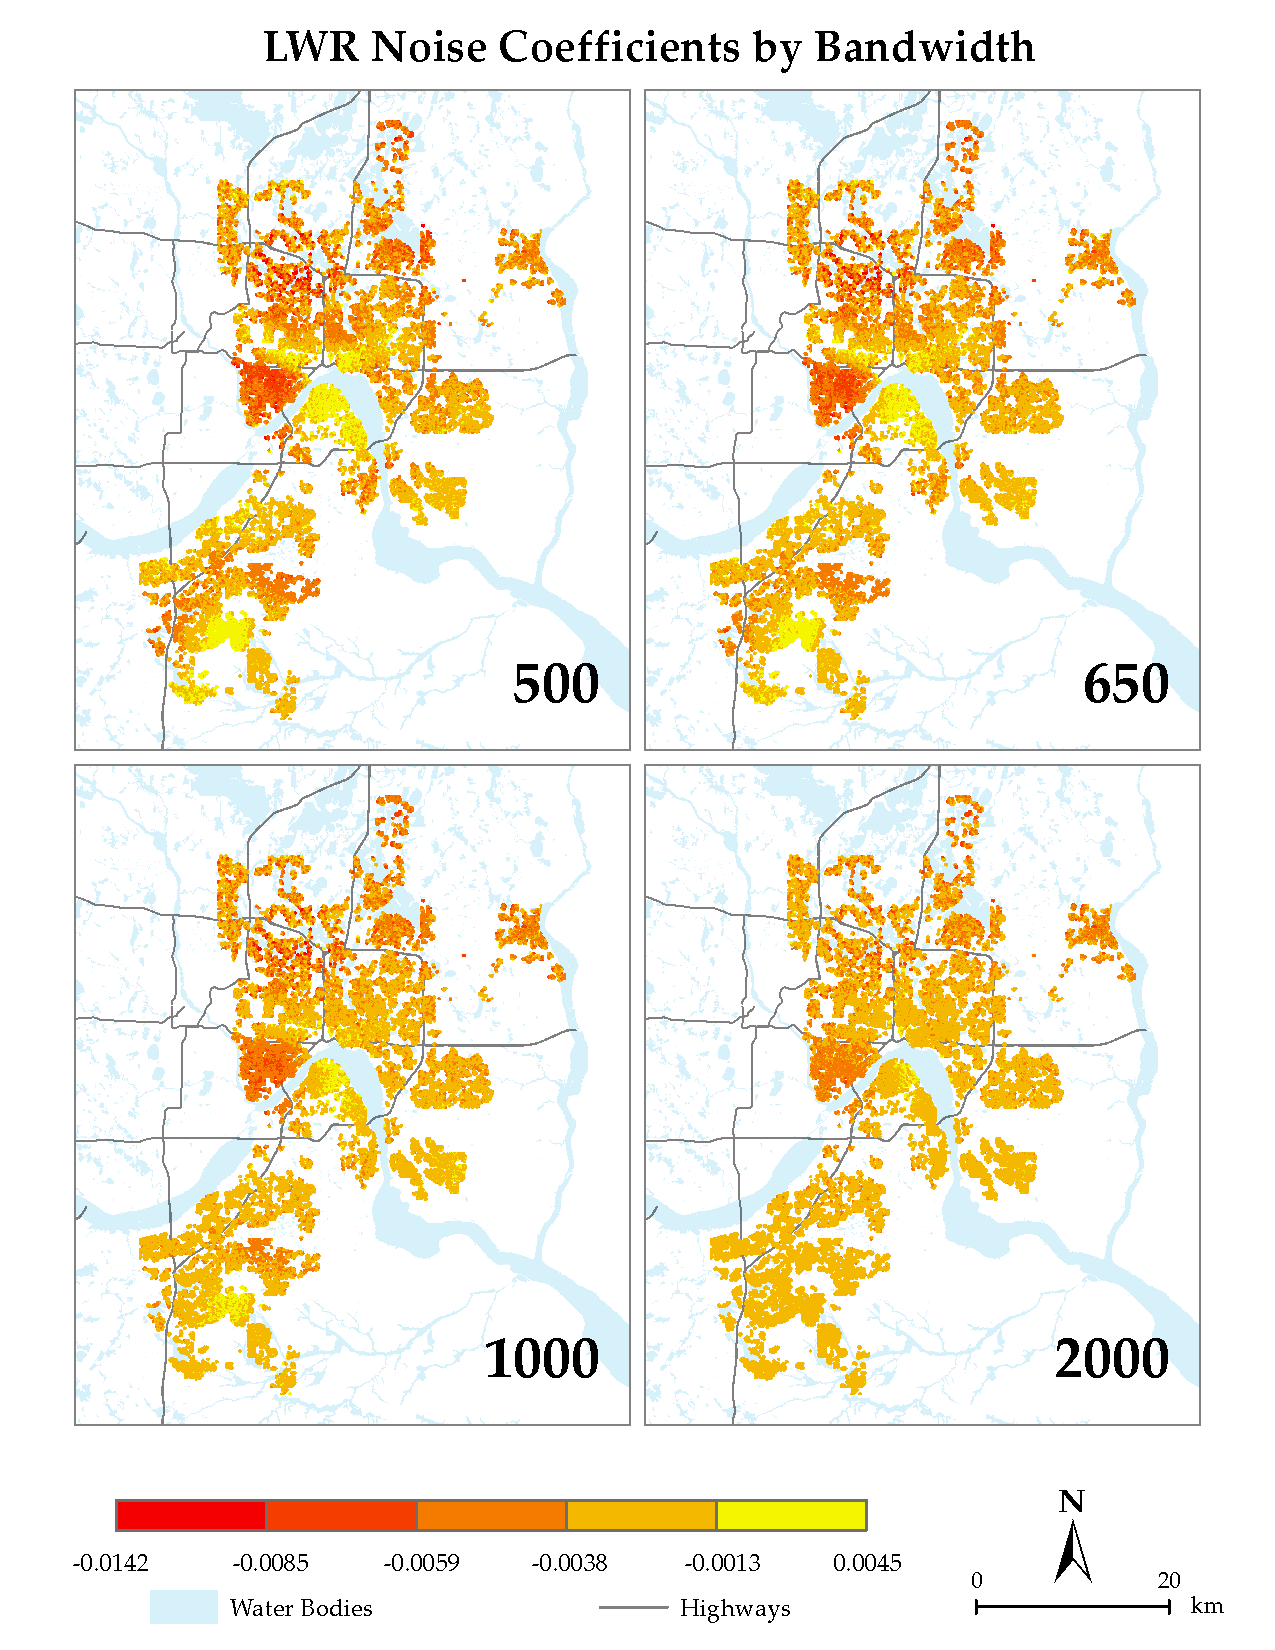
\includegraphics[width=1.1\textwidth]{../graphs/NoiseBeta_allBandwidth}}
 \caption{Simula.}\label{fig:NoiseBetas}
\end{figure}

We now conduct a second series of simulation experiments aimed at testing whether the spatial variation exhibited in particular coefficients is significant or due to random chance. The mechanics of the second simulation are very similar to the those described in the previous section. We randomly change the spatial arrangment of our house sales and estimate the LWR model. However, in this simulation we restrict the model to small bandwidths and compare the spread of the regression coefficient estimates under the random arrangment of the data to the spread found in our original LWR models with the actual spatial arrangement. If an independent variable in our hedonic regression function exhibits a stationary relationship with sales prices, then we should see similar levels of dispersion in the randomly arranged data as in our true data. However, if the dispersion we see in our random data is \emph{smaller} than the spread we observed in our actual data, that is evidence consistent with the variable having a non-stationary relationship. That is, the variation in regression coefficients obtained in our data is higher than we would observe from random chance. 

We present the results of this simulation for the same three different bandwidths in Table~\ref{tab:LWR}- 500, 650, and 1,000 nearest observations. Figures~\ref{fig:MCsds500} and \ref{fig:MCsds500} visualize the results of the second simulation for different bandwidths. Each sub-figure displays the distribution of LWR coefficient standard deviations obtained from the 100 iterations of the Monte Carlo simulation and the standard deviation obtained with the actual data (in red). Note that it is the case that the standard deviations obtained with the actual data are typically substantially larger than those obtained in the simulation for most of the variables. However, the variation obtained in the noise coefficients simulations is not dissimilar to our actual LWR results, suggesting that the spatial non-stationarity exhibited in this coefficient is perhaps due to chance and not true spatial non-stationarity in the noise coefficient. 

\begin{figure}
 \makebox[\textwidth][c]{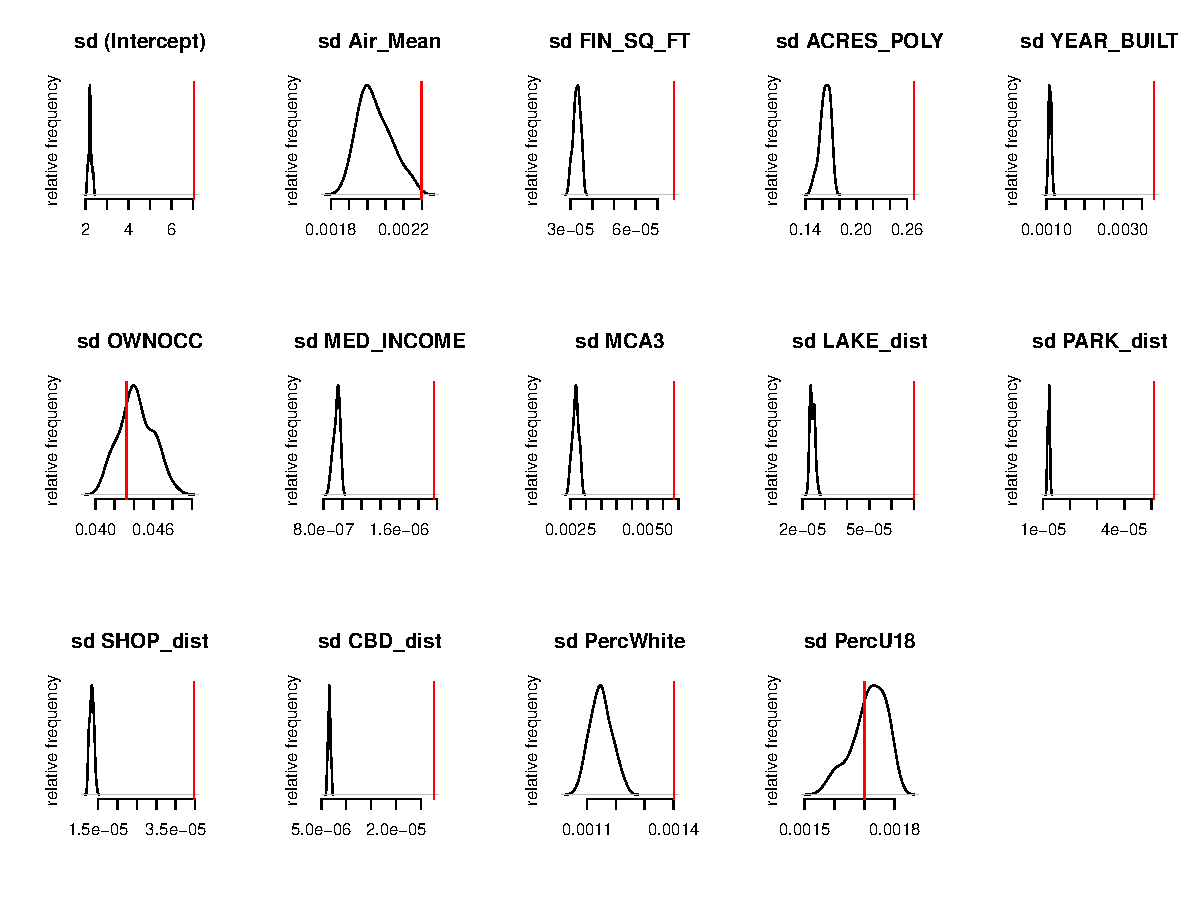
\includegraphics[width=1.2\textwidth]{../graphs/MCsimResultsSDs500}}
 \caption{Simulation Results for nearest 500 observations. Actual LWR Coefficient Standard Deviations \textcolor{red}{(red line)} vs.\ Distribution of Monte Carlo Simulation Standard Deviations by Variable. Figures in which the red line is to the right of the black distribution suggest spatial non-stationarity in effect of the variable on house prices in our study region.}\label{fig:MCsds500}
\end{figure}

\begin{figure}
 \makebox[\textwidth][c]{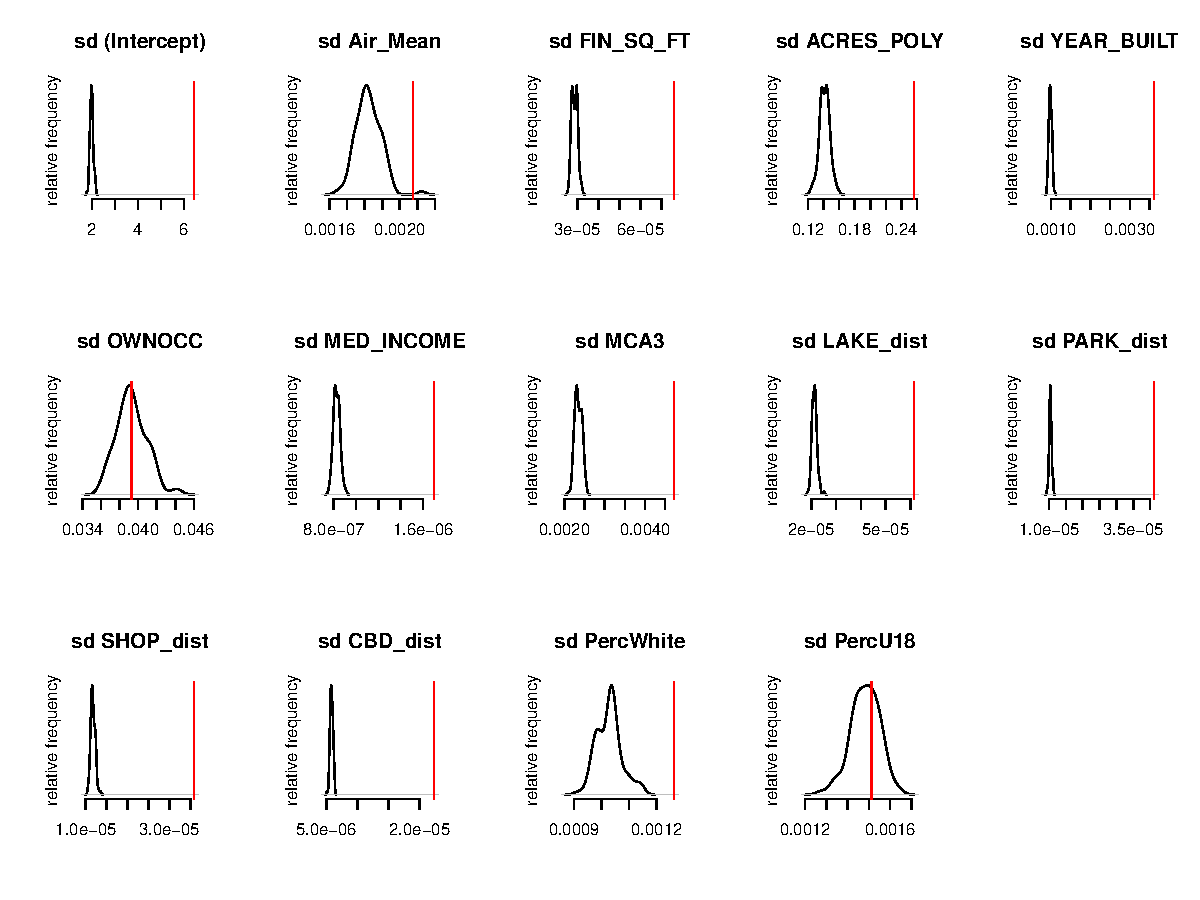
\includegraphics[width=1.2\textwidth]{../graphs/MCsimResultsSDs650}}
 \caption{Simulation Results for nearest 650 observations. Actual LWR Coefficient Standard Deviations \textcolor{red}{(red line)} vs.\ Distribution of Monte Carlo Simulation Standard Deviations by Variable. Figures in which the red line is to the right of the black distribution suggest spatial non-stationarity in effect of the variable on house prices in our study region.}\label{fig:MCsds650}
\end{figure}

[Insert figure with nearest 1,000 observations here]

\subsection{Does the Noise Coefficient Change over Time?}

Previous research has suggested that the impact of noise can change with time and economic conditions. For instance, \citet{Wilhelmsson2000} found that the traffic noise penalty to be stronger in the 1990s near Stockholm, Sweden compared to the 1980s. \citet{Cohen2009} also found the (airport) noise penalty to be larger in the early 2000s compared to the late 1990s in Atlanta, Georgia. We know that house prices in the United States fell dramatically during and after the Great Recession of 2008-09. We know less about the patterns of change in the hedonic price functions during and after the fall in house prices. \citet{Cho2011b} found evidence from hedonic analysis in Nashville, Tennessee, that consumers' willingness to pay for environmental amenities (such as proximity to open space and water views) decreased during the recession as compared to the previous economic boom. 

Figures~\ref{fig:AcreTime}--\ref{fig:NoiseTime} show the spatial distribution of some our LWR hedonic coefficients for bandwidths of 500 and 2,000 nearest sales within the last year for the sale years 2006--2010. Regardless of bandwidth, the figures show that the estimated LWR coefficients are different over time. In particular, the lot size and house size coefficients tend to decrease over time. What is surprising, however, is that the negative noise coefficient estimates tend to be more negative in later years of our study. Figure~\ref{fig:NoiseTime} shows that the spatial patterns are similar across years (the most negative coefficients tend to be in the same locations across years), but the average noise coefficient tends to be more negative for the later years.

\begin{sidewaysfigure}
 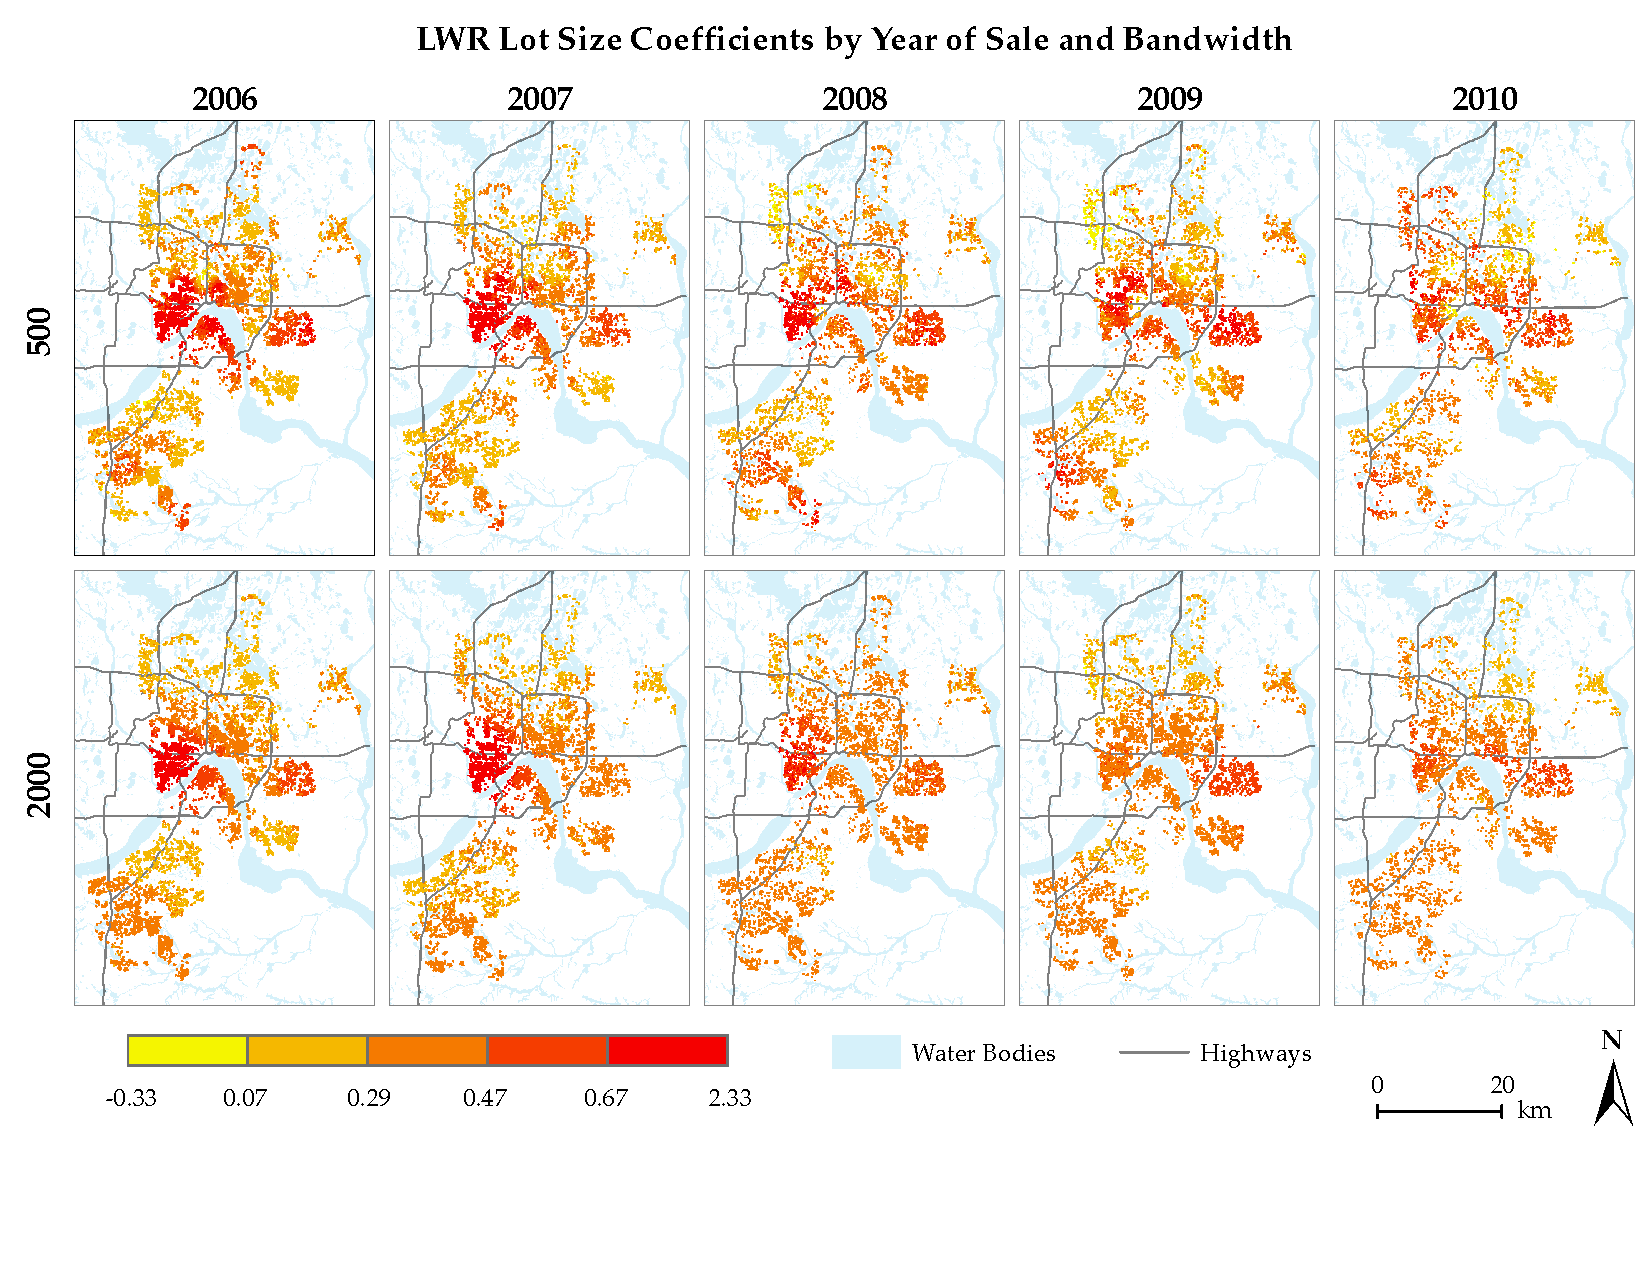
\includegraphics[trim = 0cm 2cm 0cm 0cm, clip = true, width = \textwidth]{../graphs/Acre_50_200_ByYear}
 \caption{Simula.}
 \label{fig:AcreTime}
\end{sidewaysfigure}

\begin{sidewaysfigure}
 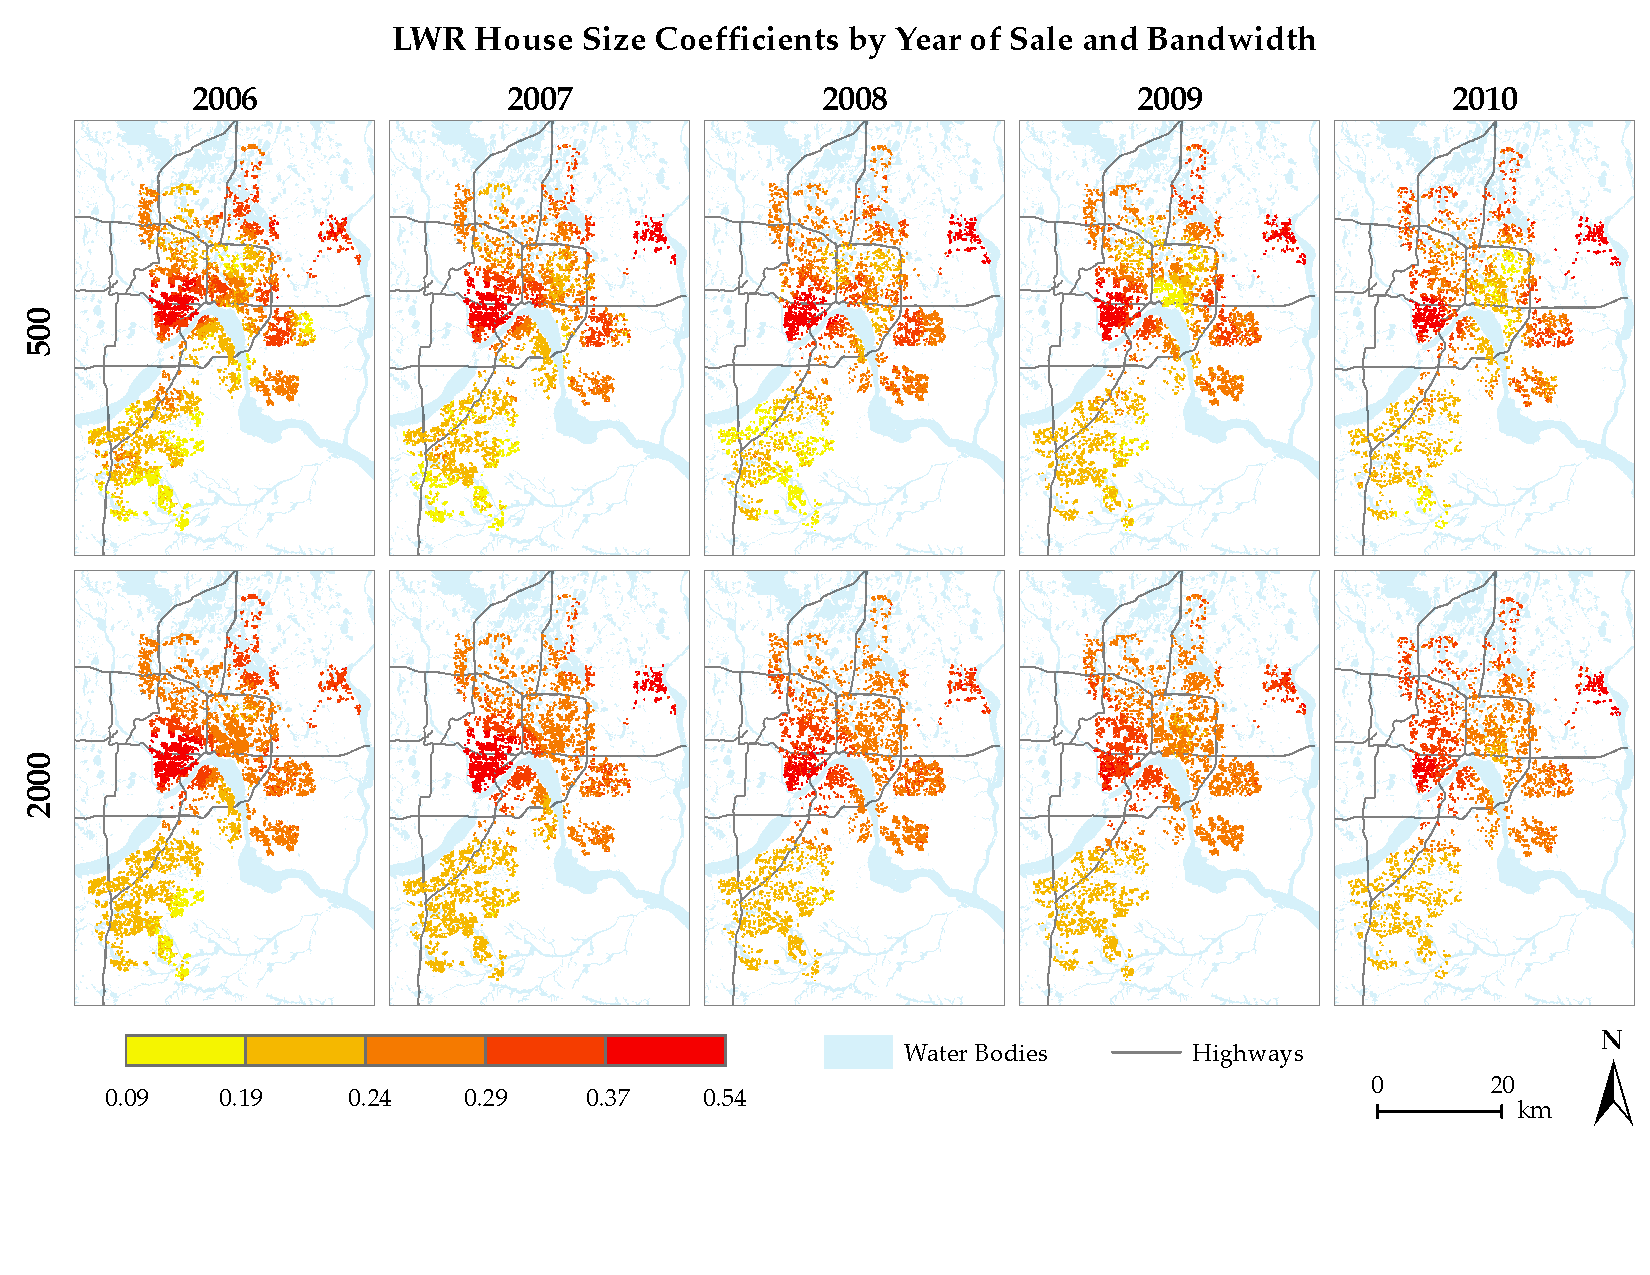
\includegraphics[trim = 0cm 2cm 0cm 0cm, clip = true, width = \textwidth]{../graphs/FinFt_50_200_ByYear}
 \caption{Simula.}
 \label{fig:HouseTime}
\end{sidewaysfigure}


\begin{sidewaysfigure}
 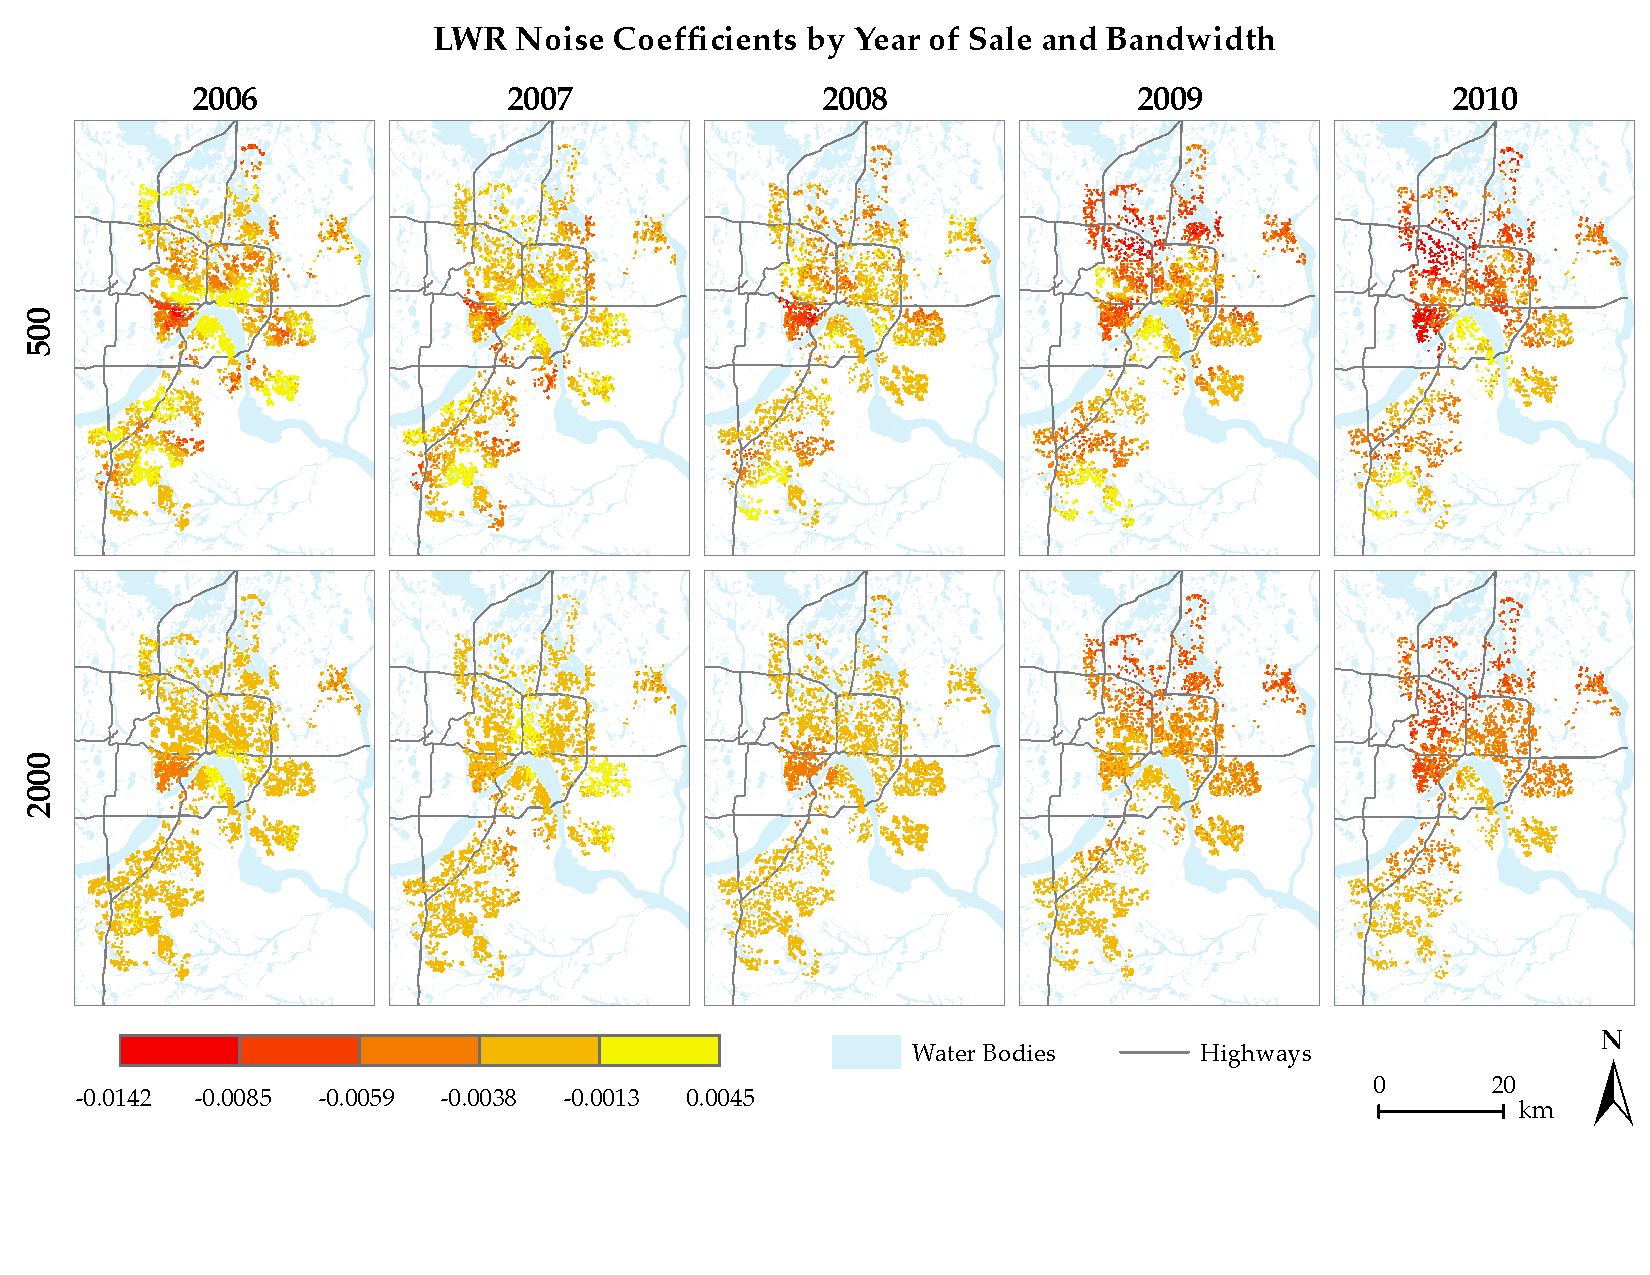
\includegraphics[trim = 0cm 2cm 0cm 0cm, clip = true, width = \textwidth]{../graphs/Noise_50_200_ByYear}
 \caption{Simula.}
 \label{fig:NoiseTime}
\end{sidewaysfigure}

We also find statistical evidence consistent with the estimated noise coefficients being more negative in the later time periods. This finding is robust to multiple different formulations and specifications. Tables~\ref{tab:noisebetatime500} and \ref{tab:noisebetatime2000} present the results of regressions using our estimated LWR noise coefficient as the dependent variable and time and spatial characteristics as explanatory variables for LWR bandwidths of 500 and 2,000 nearest sales.

Both tables are structured similarly. Column (1) finds evidence of a negative linear trend in the LWR noise coefficients over time - predicting a LWR noise coefficient of approximately twice the magnitude for the end of our study period as for the beginning. Column (2) includes a quadratic term and again predicts noise coefficients much more negative towards the end of our study period compared to the beginning. We repeat the regressions from (1) and (2) in (3) and (4) but this time also include city fixed effects in order to control for any potential locational differences of house transactions over time. Again, we see very similar results - the noise coefficient is more negative in later time periods. We also limit our analysis to just the city of St.\ Paul and repeat the analysis from (1) and (2) in columns (5) and (6). Again, we estimate the noise coefficient to be more negative in later time periods.

% Requires LaTeX packages: dcolumn 
\begin{table}[!htbp] \centering 
  \label{tab:noisebetatime500} 
\scriptsize 
\begin{tabular}{@{\extracolsep{-1pt}}lD{.}{.}{6} D{.}{.}{7} D{.}{.}{7} D{.}{.}{7} D{.}{.}{7} D{.}{.}{7} } 
\\[-1.8ex]\hline 
\hline \\[-1.8ex] 
 & \multicolumn{6}{c}{\textit{Dependent variable: LWR Noise Coefficients (bandwidth = 500 nearest sales)}} \\ 
\cline{2-7} 
\\[-1.8ex] & \multicolumn{1}{c}{(1)} & \multicolumn{1}{c}{(2)} & \multicolumn{1}{c}{(3)} & \multicolumn{1}{c}{(4)} & \multicolumn{1}{c}{(5)} & \multicolumn{1}{c}{(6)}\\ 
\hline \\[-1.8ex] 
Months since Jan 2005 & -0.00005^{***} & 0.00003^{***} & -0.00005^{***} & 0.00003^{***} & -0.0001^{***} & 0.00004^{***} \\ 
  & (0.000001) & (0.000004) & (0.000001) & (0.000004) & (0.000002) & (0.00001) \\ 
  & & & & & & \\ 
 (Months since Jan 2005)$^2$ &  & -0.000001^{***} &  & -0.000001^{***} &  & -0.000001^{***} \\ 
  &  & (0.00000005) &  & (0.00000004) &  & (0.0000001) \\ 
  & & & & & & \\ 
 Constant & -0.0016^{***} & -0.0028^{***} & -0.0021^{***} & -0.0033^{***} & -0.0015^{***} & -0.0032^{***} \\ 
  & (0.00003) & (0.0001) & (0.00003) & (0.0001) & (0.0001) & (0.0002) \\ 
  & & & & & & \\ 
\hline \\[-1.8ex] 
City Fixed Effects & \multicolumn{1}{c}{No} & \multicolumn{1}{c}{No} & \multicolumn{1}{c}{Yes} & \multicolumn{1}{c}{Yes} & \multicolumn{1}{c}{No} & \multicolumn{1}{c}{No} \\ 
\hline \\[-1.8ex] 
Observations & \multicolumn{1}{c}{31,737} & \multicolumn{1}{c}{31,737} & \multicolumn{1}{c}{31,737} & \multicolumn{1}{c}{31,737} & \multicolumn{1}{c}{8,003} & \multicolumn{1}{c}{8,003} \\ 
R$^{2}$ & \multicolumn{1}{c}{0.1273} & \multicolumn{1}{c}{0.1377} & \multicolumn{1}{c}{0.2931} & \multicolumn{1}{c}{0.3028} & \multicolumn{1}{c}{0.1566} & \multicolumn{1}{c}{0.1704} \\ 
\hline 
\hline \\[-1.8ex]  
\end{tabular} 
  \caption{LWR Noise Coefficient Over Time} 
\end{table} 

% Requires LaTeX packages: dcolumn 
\begin{sidewaystable}[!htbp] \centering 
  \caption{LWR Noise Coefficient Over Time} 
  \label{tab:noisebetatime2000} 
\scriptsize 
\begin{tabular}{@{\extracolsep{-1pt}}lD{.}{.}{6} D{.}{.}{7} D{.}{.}{7} D{.}{.}{7} D{.}{.}{7} D{.}{.}{7} } 
\\[-1.8ex]\hline 
\hline \\[-1.8ex] 
 & \multicolumn{6}{c}{\textit{LWR bandwidth = 2,000 nearest sales}} \\ 
\cline{2-7} 
\\[-1.8ex] & \multicolumn{1}{c}{(1)} & \multicolumn{1}{c}{(2)} & \multicolumn{1}{c}{(3)} & \multicolumn{1}{c}{(4)} & \multicolumn{1}{c}{(5)} & \multicolumn{1}{c}{(6)}\\ 
\hline \\[-1.8ex] 
Months since Jan 2005 & -0.00005^{***} & 0.00003^{***} & -0.00005^{***} & 0.00003^{***} & -0.00005^{***} & 0.0001^{***} \\ 
  & (0.0000003) & (0.000002) & (0.0000003) & (0.000002) & (0.000001) & (0.000004) \\ 
  & & & & & & \\ 
 (Months since Jan 2005)$^2$ &  & -0.000001^{***} &  & -0.000001^{***} &  & -0.000001^{***} \\ 
  &  & (0.00000002) &  & (0.00000002) &  & (0.0000001) \\ 
  & & & & & & \\ 
 Constant & -0.0014^{***} & -0.0026^{***} & -0.0016^{***} & -0.0028^{***} & -0.0016^{***} & -0.0033^{***} \\ 
  & (0.00001) & (0.00003) & (0.00002) & (0.00003) & (0.00003) & (0.0001) \\ 
  & & & & & & \\ 
\hline \\[-1.8ex] 
City Fixed Effects & \multicolumn{1}{c}{No} & \multicolumn{1}{c}{No} & \multicolumn{1}{c}{Yes} & \multicolumn{1}{c}{Yes} & \multicolumn{1}{c}{No} & \multicolumn{1}{c}{No} \\ 
\hline \\[-1.8ex] 
Observations & \multicolumn{1}{c}{31,737} & \multicolumn{1}{c}{31,737} & \multicolumn{1}{c}{31,737} & \multicolumn{1}{c}{31,737} & \multicolumn{1}{c}{8,003} & \multicolumn{1}{c}{8,003} \\ 
R$^{2}$ & \multicolumn{1}{c}{0.3828} & \multicolumn{1}{c}{0.4142} & \multicolumn{1}{c}{0.5128} & \multicolumn{1}{c}{0.5435} & \multicolumn{1}{c}{0.3454} & \multicolumn{1}{c}{0.3988} \\ 
\hline 
\hline \\[-1.8ex] 
\end{tabular} 
\end{sidewaystable} 

\section{Discussion}\label{Discussion}

The hedonic analysis results presented suggest that traffic noise exhibits a significant negative effect on house prices and that the hedonic function varies over space and time. These results and analysis rest on important assumptions, which if violated, may change the results. This section describes three important considerations needed to contextualize our results and worthy of discussion: causation vs.\ correlation, potential temporal problems with our data, and omitted variable bias.

In a stronger research design, we would observe the same houses over time and randomly ``treat'' some houses with more or less noise to observe the change in price relative to the control houses. Such a study is not feasible and we are therefore limited to a hedonic analysis with observational data. Our conclusions, then, should be interpretted like most other hedonic analysis results and, while we find a strong negative correlation between noise and house prices, we cannot definitely state that noise causes lower sales prices. 

Future work may want to further investigate this correlation for more evidence consistent with causation. For instance, by collecting data on the quality of house windows one could test for differential effects of more soundproof windows in noisier areas vs. quieter areas. Unfortunately, such house characteristics are unavailable for this study.

Our work faces other data limitations. Notably, while our house sales data are collected over the course of six years, the traffic noise estimates are for the year 2007. To the extent that traffic flows and composition significantly changed over time, our traffic noise variables may be inaccurate for those other time periods. However, Table VM2 from the US. Department of Transportation Office of Highway Policy Information website reports that in the year 2007 there were approximately 30 million vehicle miles traveled in the urban areas of the state of MN, while for years 2008, 2009, and 2010 the respective values were 32.5, 32.3, and 32.0. Overall, this represents a change of less than 10 percent. \footnote{\url{http://www.fhwa.dot.gov/policyinformation/quickfinddata/qftravel.cfm}} Such small changes in total vehicle miles traveled are unlikely to yield significant differences in noise levels. Additionally, we do not believe the changes are likely to manifest in significant spatial variation in traffic noise, which is ultimately responsible for our identification of the noise regression coefficient. However, given enough time for changes in driving habits and technological advancements to gain significant market penetration (for instance, quieter hybrid cars), future work should seek to create time-series noise data in order to obtain even better estimates of the impact of traffic noise over time. Given the computational complexity of re-estimating the landscape noise surface, such work is beyond the scope of this paper, but may be a worthwhile investment for future work seeking to test the robustness of our results.

Our previously reported results also lack some important control variables in the hedonic function. For instance, locations exposed to more noise due to their proximity to high traffic areas may also be less safe due to the potential for accidents. Without including a proxy variable for safety, our noise coefficient could be biased - making it appear that home prices are reflecting noise exposure when in fact it could be safety issues. Future research aimed at measuring the impact of noise should continue to seek out and control for other confounding variables. 

Our data also omits other variables and to the extent that structural variables like the number of bedrooms, bathrooms, garage size, or construction quality co-vary with other variables in our dataset, our regression coefficients will suffer from omitted variable bias. We are comforted, however, because we do have some of these important additional variables for a subset of our data. We were able to obtain the number of bedrooms, bathrooms, and garage area for our houses located within Dakota County from the Dakota County Assessor's Office. Our LWR analysis was then repeated on this geographic subset of the data in order to compare our noise coefficients across the different models. We found strikingly similar traffic noise coefficient estimates when these additional structural variables were included and omitted. As shown in Figure~\ref{fig:DAK}, a simple linear regression of the noise coefficient estimates obtained when these additional structural variables were excluded on the estimates obtained when these variables were included yields a line of best fit that is almost indiscernable from the 45 degree line and has $R^2 = 0.96$. %Additionally, a paired t-test of the roughly 9,000 (n = 8,751) coefficient estimates yields a 95 percent confidence interval for the true difference between our estimates without the additional variables and with as -0.000175 to -0.000159. That is, the estimated difference is, on average, more than an order of magnitude smaller than our typical coefficient estimates  suggesting that our results may be robust to the omission of these variables from our analysis.

\begin{figure}
\makebox[\textwidth][c]{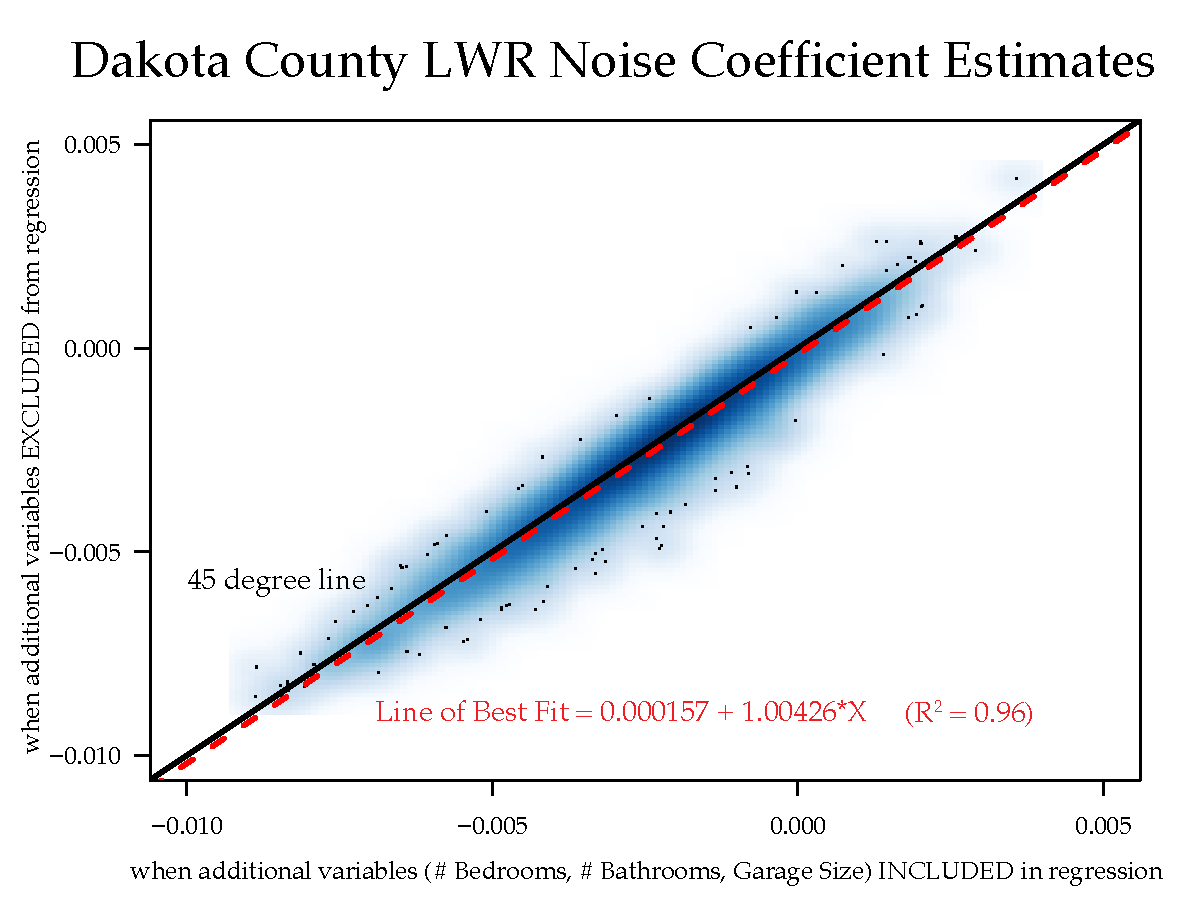
\includegraphics[width = \textwidth]{../graphs/DakotaResults}}
\caption{This figure shows the similarity between the LWR coefficients we obtained from our model in Dakota County when additional structural variables were excluded vs.\ included in the hedonic regression function. The black line shows the 45 degree line, while the red dashed line shows the estimated line of best fit, which yields a simple $R^2$ of 0.96}\label{fig:DAK}
\end{figure}

\section{Conclusion}
We estimated a hedonic price function for single family houses using Locally Weighted Regression techniques in the St.\ Paul, Minnesota, urban area. Specifically, we estimated semi-logarithmic regressions at each house within our dataset using only information contained in ``local'' (both geographically and temporally) house sales. We find strong evidence that the hedonic function in our study area varies over space and time and such flexible models represent significant improvements over conventional parametric models. 

Monte Carlo simulations suggest that the better goodness-of-fit provided by the local models are not due to chance and that many hedonic implicit prices vary over space within our study area. When the location of our data was randomly assigned and our LWR model was re-estimated across more than a dozen different bandwidths, in 100 consecutive simulations the smallest GCV score was obtained when the data were analyzed at a pooled/global level rather than local. That is, after trying thousands of different combinations of varying levels of local analysis with the spatially redistributed data, we never came close to estimating our observed housing sales prices as well as we can with the local analysis on the actual data. Additionally, re-estimating the LWR model using local bandwidths but randomly assigned locations yielded substantially smaller standard deviations for the majority of our regression coefficients. Such differences suggest that the variation exhibited by most of our regression coefficients was not due to simple random chance, but instead is consistent with spatial non-stationarity. 

While our results show very strong evidence that the coefficients on lot size and living space vary over space, the noise coefficient was one of a few variables to exhibit similar standard deviations to the simulated distributions obtained from Monte Carlo experiments. We do, however, find significant temporal variation in the impact of traffic noise in our data.

Precise estimates of the impact of traffic noise are important for efficient implementation of noise mitigation projects. The US Federal Highway Administration reports that 47 states have constructed noise barriers to reduce noise propagation, spending over a half a billion dollars from 2008-2010 \citepalias{USFHA2012}. \citet{Delucchi1998} used an estimate of 0.85 percent reduction in house prices per additional decibel in their cost-benefit analysis of traffic noise. While their preferred estimate of the total damage cost to the United States in 1991 is \$3 billion, they report a possible range of less than \$100 million to over \$40 billion due in part to uncertainty surrounding the degree of noise propagation over space in the urban built environment and the effect of noise on house prices. Indeed, one of the main conclusions of their work is that more research should be done to better understand the impact of noise on house prices and that better noise data are needed for such work to occur. 

Future research should be conducted in more housing markets, as the potential to apply the results of analysis in one set of geographical and economic circumstances may be limited. Second, ``mixed'' regression techniques (in which some regression coefficients are constrained to remain constant across the study area while others are allowed to vary) may allow researchers to obtain more precise estimates of the impact of hedonic characteristics by increasing the degrees of freedom in the regression. Future work may also seek to re-estimate traffic noise models over time to better account for changes in traffic flows associated with macroeconomic conditions. Lastly, researchers should take advantage of the recent suggestions in \citet{Carruthers2010} and use the spatial variation in regression coefficients obtained from LWR models to estimate the second-stage hedonic regressions to identify consumer demand curves for these characteristics.




\newpage
\begin{singlespace}
\bibliographystyle{plainnat}
\bibliography{NoiseBibliography}
\end{singlespace}
\end{document}
